\setcounter{exercisegroup}{7}
\edef\CurrentExerciseGroup{\arabic{exercisegroup}}
\section*{\texorpdfstring{\S\CurrentExerciseGroup}{Section \CurrentExerciseGroup}}
\phantomsection
\addcontentsline{toc}{section}{\texorpdfstring{Exercises for \S\CurrentExerciseGroup}{Exercises for Section \CurrentExerciseGroup}}

\begin{enumerate}
\def\labelenumi{\arabic{enumi})}
\tightlist
\item
  \begin{enumerate}
  \def\labelenumii{\alph{enumii})}
  \tightlist
  \item
    Let \(\mathbf{K}\) be a compact convex subset of a Hausdorff locally convex space \(\mathbf{E}\) , \(\mu\) a positive measure on \(\mathbf{K}\) of mass 1, \(\mathbf{b}_{\mu}\) its barycenter. Show that for every positive function \(f\) on \(\mathbf{K}\) that is concave and lower semi-continuous, one has \(f(\mathbf{b}_{\mu}) \geqslant \int^{*} f d\mu\) . (Note that \(f\) is bounded (TVS, II, §2, Exer. 32), consequently \(-f\) is \(\mu\) -integrable.) From this, conclude that if \(f\) is a lower semi-continuous (or upper semi-continuous) function on \(\mathbf{K}\) that is both convex and concave, then \(\int f d\mu = f(\mathbf{b}_{\mu})\) .
  \end{enumerate}
\end{enumerate}

\begin{enumerate}
\def\labelenumi{\alph{enumi})}
\setcounter{enumi}{1}
\tightlist
\item
  Let I be the interval \([0,1]\) of R, K the subset of \(\mathcal{M}_{+}(I)\) formed by the positive measures of total mass 1, which is convex and compact for the vague topology, and let \(j: x \mapsto \varepsilon_{x}\) be the canonical injection of I into K, which is a homeomorphism of I onto a subspace of K. For every measure \(\nu \in K\) , set \(g(\nu) = \sum_{x \in I} \nu(\{x\})\) ; this is a function that
\end{enumerate}

is both convex and concave in K; moreover, if \(g_{n}(\nu)\) is the supremum of the \(\nu(A)\) for all the finite subsets A of I having at most n elements, then \(g_{n}\) is upper semi-continuous on K, and \(g(\nu) = \lim_{n \to \infty} g_{n}(\nu)\) for every \(\nu \in K\) , therefore g is \(\lambda\) -integrable for every measure \(\lambda\) on K. Let \(\mu\) be the measure on K such that \(\int f d\mu = \int_{\mathrm{I}} f(j(x)) dx\) for \(f \in \mathcal{K}(\mathrm{X}; \mathbf{R})\) , which is positive and of total mass 1; show that \(\mathbf{b}_{\mu}\) is Lebesgue measure on I and that \(\int g d\mu \neq g(\mathbf{b}_{\mu})\) .

\begin{enumerate}
\def\labelenumi{\arabic{enumi})}
\setcounter{enumi}{1}
\tightlist
\item
  Let X be a compact space, P a set of lower semi-continuous numerical functions on X, taking values in \(]-\infty,+\infty]\) . Assume that P contains the finite constants; for every function \(h\in P\) and every positive measure \(\mu\) on X, \(\mu^{*}(h)\) is defined and \(>-\infty\) (§4, Exer. 5).
\end{enumerate}

\begin{enumerate}
\def\labelenumi{\alph{enumi})}
\item
  For two positive measures \(\mu, \nu\) on \(X\) , write \(\mu \prec \nu\) if \(\mu^{*}(h) \leqslant \nu^{*}(h)\) for every function \(h \in \mathcal{P}\) . Show that the relation \(\mu \prec \nu\) is a pre-order relation on \(\mathcal{M}_{+}(X)\) ; it implies that \(\mu(1) = \nu(1)\) , \(c\mu \prec c\nu\) for all \(c > 0\) , and \(\mu + \lambda \prec \nu + \lambda\) for every measure \(\lambda \in \mathcal{M}_{+}(X)\) .
\item
  Assume that \(\mathcal{P} + \mathcal{P} \subset \mathcal{P}\) and that \(c \cdot \mathcal{P} \subset \mathcal{P}\) for \(c > 0\) . Let \(\mu\) be a positive measure on \(X\) , \(f\) a function in \(\mathcal{C}(X; \mathbf{R})\) . Denote by \(Q_f\) the set of functions \(h \geqslant f\) belonging to \(\mathcal{P}\) , and by \(M_\mu\) the set of measures \(\lambda \in \mathcal{M}_+(X)\) such that \(\lambda \prec \mu\) . Show that
\end{enumerate}

\[
\sup _ {\lambda \in \mathrm{M} _ {\mu}} \lambda (f) = \inf _ {h \in \mathrm{Q} _ {f}} \mu^ {*} (h).
\]

(For every function \(g \in \mathcal{C}(\mathrm{X};\mathbf{R})\) , let \(p(g) = \inf_{h \in \mathrm{Q}_g} \mu^*(h)\) . Show that \(p(g + g') \leqslant p(g) + p(g')\) and \(p(cg) = c \cdot p(g)\) for \(g, g'\) in \(\mathcal{C}(\mathrm{X};\mathbf{R})\) and \(c > 0\) ; prove on the other hand that \(\mathrm{M}_{\mu}\) is identical to the set of measures \(\lambda \in \mathcal{M}_{+}(\mathrm{X})\) such that, for every function \(g \in \mathcal{C}(\mathrm{X};\mathbf{R})\) , one has \(\lambda(g) \leqslant p(g)\) , and conclude by applying the Hahn-Banach theorem.) If the functions in \(\mathcal{P}\) are continuous and if \(S_0(f)\) is the lower envelope of \(Q_f\) , then also \(\mu(S_0(f)) = \sup \lambda(f)\) .

\[
\lambda \in \mathrm{M} _ {\mu}
\]

\begin{enumerate}
\def\labelenumi{\alph{enumi})}
\setcounter{enumi}{2}
\item
  If the set \(\mathcal{P}_0\) of functions in \(\mathcal{P}\) that are continuous and finite on X is total in \(\mathcal{C}(\mathrm{X};\mathbf{R})\) , then the relation \(\mu \prec \nu\) is an order relation on \(\mathcal{M}_{+}(\mathrm{X})\) . If a measure \(\nu \in \mathcal{M}_{+}(\mathrm{X})\) is maximal for this order relation, then so is every measure \(\nu'\) such that \(0 \leqslant \nu' \leqslant \nu\) (for the usual order) (argue by contradiction using \(a\) )). If \(\mathcal{P}_0 = \mathcal{P}\) and \(\mathcal{P}\) is total, then every increasing directed set for the order relation \(\mu \prec \nu\) admits a supremum in \(\mathcal{M}_{+}(\mathrm{X})\) for this relation; in particular, \(\mathcal{M}_{+}(\mathrm{X})\) is inductive for this relation.
\item
  Suppose that the functions in \(\mathcal{P}\) are continuous and finite, that \(\mathcal{P}\) is total in \(\mathcal{C}(\mathrm{X};\mathbf{R})\) , and that \(\mathcal{P} + \mathcal{P} \subset \mathcal{P}\) and \(c \cdot \mathcal{P} \subset \mathcal{P}\) for all \(c > 0\) . For every function \(f \in \mathcal{C}(\mathrm{X};\mathbf{R})\) , denote by \(\mathrm{S}(f)\) the lower envelope of the functions \(h \in -\mathcal{P}\) such that \(f \leqslant h\) ; for every \(\varepsilon > 0\) , denote by \(\mathrm{K}_{f,\varepsilon}\) the set of \(x \in \mathrm{X}\) such that \(\mathrm{S}(f)(x) \geqslant f(x) + \varepsilon\) . Show that the following conditions are equivalent:
\end{enumerate}

\(\alpha)\) The measure \(\mu \in \mathcal{M}_{+}(\mathrm{X})\) is maximal for the order relation \(\lambda \prec \lambda'\) .

\(\beta)\) For every function \(f \in \mathcal{C}(\mathrm{X}; \mathbf{R})\) , \(\mu(\mathrm{S}(f)) = \mu(f)\) .

\(\beta^{\prime})\) For every function \(f \in \mathcal{P}\) , \(\mu(\mathrm{S}(f)) = \mu(f)\) .

\(\gamma)\) For every function \(f \in \mathcal{C}(\mathrm{X}; \mathbf{R})\) and every \(\varepsilon > 0\) , \(\mu(\mathrm{K}_{f,\varepsilon}) = 0\) .

\(\gamma^{\prime})\) For every function \(f\in \mathcal{P}\) and every \(\varepsilon >0\) , \(\mu (\mathrm{K}_{f,\varepsilon}) = 0\)

(Apply b) to \(-\mathcal{P}\) .)

\begin{enumerate}
\def\labelenumi{\alph{enumi})}
\setcounter{enumi}{4}
\tightlist
\item
  Under the hypotheses of \(d\) ), show that if \(\mu\) and \(\mu'\) are two positive measures on \(X\) that are maximal for the relation \(\prec\) , then so is \(\mu + \mu'\) . From this, deduce that the set of positive measures that are maximal for this order relation is a lattice for the usual order relation \(\leqslant\) .
\end{enumerate}

¶ 3) Let X be a nonempty compact space, P a set of lower semi-continuous numerical functions on X, taking values in \([-\infty, +\infty]\) ; assume that P contains the finite constants. A point \(x \in X\) is said to be P-extremal if the measure \(\varepsilon_{x}\) is minimal for the pre-order relation \(\mu \prec \nu (*)\) ; the set of P-extremal points is denoted \(\mathrm{Ch}_{\mathcal{P}}(\mathrm{X})\) .

\begin{enumerate}
\def\labelenumi{\alph{enumi})}
\tightlist
\item
  Show that if \(\mathcal{P}'\) is the set of linear combinations \(\sum_{i} c_i h_i\) of functions in \(\mathcal{P}\)
\end{enumerate}

with coefficients \(\geqslant 0\) , the \(\mathcal{P}\) -extremal points are identical to the \(\mathcal{P}'\) -extremal points.

\begin{enumerate}
\def\labelenumi{\alph{enumi})}
\setcounter{enumi}{1}
\tightlist
\item
  For a point \(x \in X\) , show that the following conditions are equivalent:
\end{enumerate}

\(\alpha)\) \(x\) is \(\mathcal{P}\) -extremal.

\(\beta)\) For every function \(f \in \mathcal{C}(\mathrm{X}; \mathbf{R})\) and every \(\varepsilon > 0\) , there exists an \(h \in \mathcal{P}'\) such that \(f \leqslant h\) and \(h(x) \leqslant f(x) + \varepsilon\) .

\(\gamma)\) For every open neighborhood U of \(x\) and every \(\varepsilon > 0\) , there exists a function \(h \geqslant 0\) in \(\mathcal{P}'\) such that \(h(x) \leqslant \varepsilon\) and \(h(y) \geqslant 1\) for all \(y \in X - U\) . (Use Exer. 2 b.)

Show, moreover, that the set of points of \(\mathrm{Ch}_{\mathcal{P}}(\mathrm{X})\) where at least one function in \(\mathcal{P}\) attains its infimum in \(\mathrm{X}\) is dense in \(\mathrm{Ch}_{\mathcal{P}}(\mathrm{X})\) .

\begin{enumerate}
\def\labelenumi{\alph{enumi})}
\setcounter{enumi}{2}
\item
  A subset F of X is said to be P-stable if it is closed and if the relations \(\lambda \prec \mu\) and \(\operatorname{Supp}(\mu) \subset F\) imply \(\operatorname{Supp}(\lambda) \subset F\) . Show that if \(u \in P\) and if \(F'\) is the set of points of F where u attains its infimum in F, then the set \(F'\) is P-stable.
\item
  Assume in addition that \(\mathcal{P}\) separates the points of X. Show that for every function \(h \in \mathcal{P}\) , the set \(S_h\) of points of X where \(h\) attains its infimum in X intersects \(\mathrm{Ch}_{\mathcal{P}}(X)\) . (Consider a minimal \(\mathcal{P}\) -stable subset contained in \(S_h\) and use \(c\) ) to show that such a subset reduces to a single point.)
\item
  With the same hypotheses as in \(d\) ), show that for a closed subset \(\mathbf{F}\) of \(\mathbf{X}\) to contain \(\mathrm{Ch}_{\mathcal{P}}(\mathbf{X})\) , it is necessary and sufficient that for every function \(h \in \mathcal{P}'\) , \(\mathbf{F}\) intersect the set \(\mathbf{S}_h\) of points where \(h\) attains its infimum in \(\mathbf{X}\) (make use of \(b\) ). From this, deduce that for \(a \in \mathbf{X}\) to be in the closure of \(\mathrm{Ch}_{\mathcal{P}}(\mathbf{X})\) , it is necessary and sufficient that for every open neighborhood \(\mathbf{U}\) of \(a\) , there exist \(h \in \mathcal{P}'\) and \(b \in \mathbf{U}\) such that \(h(b) < h(x)\) for all \(x \in \mathbf{X} - \mathbf{U}\) (in other words, \(\mathbf{S}_h \subset \mathbf{U}\) ).
\item
  Under the hypotheses of \(d\) ), a subset A of X is said to be a \(\mathcal{P}\) -edge if, for every function \(h \in \mathcal{P}'\) , \(\mathrm{S}_h\) intersects A. Take for X the union, in \(\mathbf{R}^2\) , of the two circles with respective centers \((-1,0)\) and \((1,0)\) and with radius 1, and for \(\mathcal{P}\) the set of restrictions to X of the affine linear functions on \(\mathbf{R}^2\) . Show that \(\operatorname{Ch}_{\mathcal{P}}(\mathrm{X})\) consists of the points \((\xi, \eta)\) of X such that \(|\xi| \geqslant 1\) . If \(a\) is the \(\mathcal{P}\) -extremal point \((1,1)\) , show that there is a neighborhood U of \(a\) such that there is no function \(h \in \mathcal{P}'\) for which \(h \geqslant 0\) , \(h(a) = 0\) and \(h(y) \geqslant 1\) on \(\mathrm{X} - \mathrm{U}\) . If A and \(\mathrm{A}'\) are the complements in \(\operatorname{Ch}_{\mathcal{P}}(\mathrm{X})\) of the points \((1,1)\) and \((-1,1)\) , respectively, then A and \(\mathrm{A}'\) are \(\mathcal{P}\) -edges but the same is not true of \(\mathrm{A} \cap \mathrm{A}'\) ; thus there is no smallest \(\mathcal{P}\) -edge.
\end{enumerate}

\(g)\) Let \(\mathbf{Y}\) be a second compact space, \(\mathcal{Q}\) a set of lower semi-continuous mappings of \(\mathbf{Y}\) into \([-\infty, +\infty]\) , containing the finite constants. Let \(\mathcal{H}\) be the set of functions \(h = f \otimes g\) with \(f \in \mathcal{P}\) and \(g \in \mathcal{Q}\) ; show that \(\mathrm{Ch}_{\mathcal{H}}(\mathrm{X} \times \mathrm{Y}) = \mathrm{Ch}_{\mathcal{P}}(\mathrm{X}) \times \mathrm{Ch}_{\mathcal{Q}}(\mathrm{Y})\) .

¶ 4) Let E be a Hausdorff locally convex space, X a compact convex set in E, P the set of finite numerical functions continuous and convex in X; \(\mu \prec \nu\) denotes the pre-order relation defined on \(\mathcal{M}_{+}(X)\) by P (Exer. 2).

\begin{enumerate}
\def\labelenumi{\alph{enumi})}
\item
  Show that \(\mu \prec \nu\) is an order relation on \(\mathcal{M}_{+}(\mathrm{X})\) (use Exer. 29 of TVS, II, §5) and that, for every \(x \in \mathrm{X}\) , the relation \(\varepsilon_x \prec \mu\) is equivalent to saying that \(\mu\) has mass 1 and \(x\) is the barycenter of \(\mu\) . For every maximal measure \(\mu\) (for the preceding order relation) of mass 1, there therefore exists one and only one \(x \in \mathrm{X}\) such that \(\varepsilon_x \prec \mu\) . Conversely, every \(z \in \mathrm{X}\) is the barycenter of at least one maximal measure. For \(x \in \mathrm{X}\) to be an extremal point of \(\mathrm{X}\) , it is necessary and sufficient that \(\varepsilon_x\) be a maximal measure.
\item
  Let \(\mu\) be a maximal measure on \(\mathrm{X}\) , \(f\) a function in \(\mathcal{C}_{+}(\mathrm{X})\) . Show that for every \(\varepsilon > 0\) , there exists a continuous convex function \(g\) on \(\mathrm{X}\) such that \(0 \leqslant g \leqslant f\) and \(\mu(g) \geqslant \mu(f) - \varepsilon\) (use Exers. 3 b) and 2 d)). From this, deduce that the support of \(\mu\) is contained in the closure of the set of extremal points of \(\mathrm{X}\) .
\item
  Let \(\mu\) be a maximal measure on \(X\) , \((f_n)_{n \geqslant 1}\) a decreasing sequence of functions in \(\mathcal{C}_+(X)\) . Show that if, for every extremal point \(x \in X\) , the sequence \((f_n(x))\) tends to 0, then \(\lim_{n \to \infty} \mu(f_n) = 0\) (use \(b\) ) to construct a decreasing sequence \((g_n)\) of continuous convex functions such that \(0 \leqslant g_n \leqslant f_n\) and \(\mu(g_n) \geqslant \mu(f_n) - \varepsilon\) for all \(n\) , and show that the sequence \((g_n(y))\) tends to 0 for every \(y \in X\) ).
\item
  Deduce from c) that if \(A \subset X\) contains no extremal point and is the union of a sequence \((\mathrm{K}_{n})\) of compact subsets of X, each of which is a countable intersection of open sets in X, then \(\mu(\mathrm{A}) = 0\) for every maximal measure \(\mu\) .
\item
  Let \(\mathcal{A}\) be the vector space of continuous functions on X that are the restrictions to X of continuous affine linear functions on E. The relation \(\lambda \prec \mu\) implies that \(\lambda(h) = \mu(h)\) for every function \(h \in \mathcal{A}\) ; for every function \(f \in \mathcal{C}(\mathrm{X};\mathbf{R})\) , the lower envelope \(\mathrm{S}(f)\) of the functions \(h \in \mathcal{A}\) such that \(f \leqslant h\) is also the lower envelope of the functions \(g \in -\mathcal{P}\) such that \(f \leqslant g\) . For every \(x \in X\) , the relation \(\varepsilon_x \prec \mu\) is equivalent to the relation \(h(x) = \langle h, \mu \rangle\) for all \(h \in \mathcal{A}\) ; the extremal points of X are identical to the \(\mathcal{A}\) -extremal points. If \(f \in \mathcal{P}\) then, for every \(x \in X\) ,
\end{enumerate}

\[
\mathrm{S} (f) (x) = \sup _ {\varepsilon_ {x} \prec \mu} \int f (y) d \mu (y)\tag{*}
\]

(use Exer. 2 b)). This formula is no longer necessarily valid if it is only assumed that f is convex and upper semi-continuous on X (with the notations of Exer. 1 b), consider the function f equal to 1 on the image of I in K, and to 0 elsewhere).

\begin{enumerate}
\def\labelenumi{\alph{enumi})}
\setcounter{enumi}{5}
\tightlist
\item
  Show that the formula (*) is again valid when in the second member one limits oneself to the discrete measures \(\mu\) having x as barycenter.
\end{enumerate}

¶ 5) The notations being those of Exer. 4 e), let \(\mathcal{A}'\) denote the dual of the normed space \(\mathcal{A}\) , equipped with the order structure deduced from that of \(\mathcal{A}\) (Ch. II, §2). On the other hand, denote by C the convex cone with vertex 0 generated by \(X \times \{1\}\) in the space \(E \times R\) .

\begin{enumerate}
\def\labelenumi{\alph{enumi})}
\tightlist
\item
  Show that the following properties are equivalent:
\end{enumerate}

\begin{enumerate}
\def\labelenumi{(\roman{enumi})}
\item
  Every point \(x \in X\) is the barycenter of a unique maximal measure \(\beta_x\) of mass 1 on \(X\) .
\item
  The vector space F generated by C is a lattice for the order structure having C as the set of elements \(\geqslant0\) (in other words, X is a simplex (TVS, II, §2, Exer. 41)).
\item
  For every function \(f \in \mathcal{P}\) , \(S(f)\) is both concave and convex.
\item
  If \(\mu\) and \(\nu\) are two maximal measures such that \(\mu(h) = \nu(h)\) for all \(h \in \mathcal{A}\) , then \(\mu = \nu\) .
\item
  The vector space \(\mathcal{A}'\) is a Riesz space.
\item
  If \(f\) and \(g\) are two functions in \(\mathcal{P}\) , then \(S(f + g) = S(f) + S(g)\) .
\end{enumerate}

(First prove that (i) implies the following property:

\begin{enumerate}
\def\labelenumi{(\roman{enumi})}
\setcounter{enumi}{6}
\tightlist
\item
  The mapping \(x \mapsto \beta_{x}\) may be extended in only one way to a bijective linear mapping of F onto the subspace of \(\mathcal{M}(X)\) generated by the maximal measures, and this mapping transforms C into the cone of maximal measures.
\end{enumerate}

Then deduce (ii) from (vii), using Exer. 2 e). To deduce (iii) from (ii), use the decomposition lemma in the Riesz space F and Exer. 4 f). To deduce (iv) from (iii), use the fact that if \(g \in \mathcal{C}(X; \mathbf{R})\) is both concave and convex, then the set of \(h \in A\) such that \(h(x) > g(x)\) for all \(x \in X\) is a decreasing directed set (TVS, II, §5, Prop. 6) and has g for its lower envelope; then apply Exer. 4 e). To deduce (v) from (iv), observe that \(A'\) may be identified with the subspace of \(\mathcal{M}(X)\) generated by the maximal measures, with the help of Exer. 4 e). To deduce (vi) from (v), apply the decomposition lemma in the Riesz space \(A'\) and Exer. 4 f). Finally, to deduce (i) from (vi), consider the mapping \(f \mapsto S(f)(x)\) for \(f \in P\) and \(x \in X\) , and use Exer. 4 e).

\begin{enumerate}
\def\labelenumi{\alph{enumi})}
\setcounter{enumi}{1}
\item
  When the conditions of a) are satisfied, show that for every function \(f \in \mathcal{C}(X; \mathbf{R})\) , the mapping \(x \mapsto \beta_x(f)\) is in the closure, for the topology of uniform convergence in X, of the set of bounded functions on X that are the difference of two upper semi-continuous functions (make use of the fact that P is total in \(\mathcal{C}(X; \mathbf{R})\) ); consequently, this mapping is measurable for every measure on X. *For every positive measure \(\mu\) on X, the unique maximal measure \(\nu \succ \mu\) is given by \(\nu = \int \beta_x d\mu(x)\) (cf.~Ch. V).*
\item
  When the conditions of \(a\) ) are satisfied and X is in addition metrizable, show that for every \(x \in X\) , \(\beta_x\) is the only positive measure \(\mu\) of mass 1 and barycenter \(x\) such that \(\mu(X - L) = 0\) , where \(L\) is the set \(\mathrm{Ch}_{\mathcal{A}}(X)\) of extremal points (argue as in Th. 1).
\item
  When the conditions of a) are satisfied, show that the following properties are equivalent:
\end{enumerate}

\(\alpha)\) The set \(\mathrm{L} = \mathrm{Ch}_{\mathcal{A}}(\mathrm{X})\) is closed, in other words \(\check{\mathrm{S}}_{\mathcal{A}}(\mathrm{X}) = \mathrm{Ch}_{\mathcal{A}}(\mathrm{X})\) .

\(\beta)\) For every function \(f \in \mathcal{P}\) , the restriction of \(\mathrm{S}(f)\) to \(\overline{\mathrm{L}}\) is continuous.

\(\gamma)\) For every function \(f \in \mathcal{P}\) , the function \(S(f)\) is continuous on \(X\) .

\(\delta)\) The mapping \(x \mapsto \beta_x\) of X into \(\mathcal{M}_+(X)\) (equipped with the vague topology) is continuous.

(To show that \(\alpha\) ) implies \(\beta\) ), observe that \(\beta_x = \varepsilon_x\) in L. To prove that \(\beta\) implies \(\gamma\) ), use the fact that S(f) is the lower envelope of a decreasing directed set of functions in \(\mathcal{A}\) (TVS, II, §5, Prop. 6), Dini's theorem and Exer. 3 \(d\) ) applied to the functions in \(\mathcal{A}\) . To prove that \(\gamma\) implies \(\delta\) ), use Exer. 4 \(e\) ). Finally, to see that \(\delta\) implies \(\alpha\) ), use Exer. 4 \(a\) .)

¶ 6) Let X be a nonempty compact space, H a linear subspace of \(\mathcal{C}(X;R)\) containing the constants and separating the points of X. The relation \(\lambda \prec \mu\) defined by H (Exer. 2) is then an equivalence relation, and the points H-extremal in the sense of Exer. 3 are identical to the points H-extremal in the sense of No.~3.

Let \(\mathbf{F}\) be a closed subset of \(\mathbf{X}\) containing \(\operatorname{Ch}_{\mathcal{H}}(\mathbf{X})\) ; for every \(x \in \mathbf{X}\) , denote by \(\mathcal{M}_x^{\mathrm{F}}\) the set of positive measures \(\mu\) on \(\mathbf{X}\) , of total mass 1, such that \(\varepsilon_x \prec \mu\) and \(\operatorname{Supp}(\mu) \subset \mathbf{F}\) ; in order that \(\varepsilon_x \in \mathcal{M}_x^{\mathrm{F}}\) , it is necessary and sufficient that \(x \in \mathbf{F}\) ; the relation \(x \in \operatorname{Ch}_{\mathcal{H}}(\mathbf{X})\) is equivalent to \(\mathcal{M}_x^{\mathrm{F}} = \{\varepsilon_x\}\) . For every bounded numerical function \(f\) defined on \(\mathbf{F}\) and for every \(x \in X\) , set

\[
\overline {{\mathrm{H}}} _ {x} ^ {\mathrm{F}} (f) = \inf _ {f \leqslant h | \mathrm{F}, h \in \mathscr {H}} h (x), \quad \underline {{\mathrm{H}}} _ {x} ^ {\mathrm{F}} (f) = - \overline {{\mathrm{H}}} _ {x} ^ {\mathrm{F}} (- f) = \sup _ {f \geqslant h | \mathrm{F}, h \in \mathscr {H}} h (x),
\]

which are finite numbers.

\begin{enumerate}
\def\labelenumi{\alph{enumi})}
\item
  Show that the mapping \(f \mapsto \overline{\mathrm{H}}_x^{\mathrm{F}}(f)\) of \(\mathcal{C}(\mathrm{F};\mathbf{R})\) into \(\mathbf{R}\) is increasing, positively homogeneous and convex. If \(h \in \mathcal{H}\) , then \(\overline{\mathrm{H}}_x^{\mathrm{F}}(h) = h(x)\) .
\item
  For every \(x \in X\) , every measure \(\mu \in \mathcal{M}_x^{\mathrm{F}}\) and every function \(f \in \mathcal{C}(\mathrm{F};\mathbf{R})\) , \(\underline{\mathrm{H}}_x^{\mathrm{F}}(f) \leqslant \int f d\mu \leqslant \overline{\mathrm{H}}_x^{\mathrm{F}}(f)\) . Conversely if, for a function \(f_0 \in \mathcal{C}(\mathrm{F};\mathbf{R})\) , \(\gamma\) is a real number such that \(\underline{\mathrm{H}}_x^{\mathrm{F}}(f_0) \leqslant \gamma \leqslant \overline{\mathrm{H}}_x^{\mathrm{F}}(f_0)\) , then there exists a measure \(\mu \in \mathcal{M}_x^{\mathrm{F}}\) such that \(\gamma = \int f_0 d\mu\) .
\item
  Show that for a function \(g \in \mathcal{C}(\mathrm{X};\mathbf{R})\) , the following conditions are equivalent:
\end{enumerate}

\(\alpha)\) For every \(x \in X\) and every measure \(\mu \in \mathcal{M}_x^{\mathrm{F}}\) , one has \(g(x) = \int g d\mu\) .

\(\beta)\) For every \(x \in \mathrm{X}\) , \(\underline{\mathrm{H}}_x^{\mathrm{F}}(g|\mathrm{F}) = \overline{\mathrm{H}}_x^{\mathrm{F}}(g|\mathrm{F}) = g(x)\) .

\(\gamma)\) For every \(\varepsilon > 0\) there exist two finite sequences \((h_i'), (h_j'')\) of functions in \(\mathcal{H}\) such that, setting \(h' = \sup(h_i')\) , \(h'' = \inf(h_j'')\) , one has \(h' \leqslant g \leqslant h''\) and \(h'' - h' \leqslant \varepsilon\) .

(To see that \(\beta\) ) implies \(\gamma\) ), argue as in GT, X, §4, No.~1, Prop. 2.)

When a function \(g \in \mathcal{C}(\mathrm{X};\mathbf{R})\) has the preceding equivalent properties, it is said to be \(\mathcal{H}\) -harmonic; the set \(\mathcal{H}^c\) of \(\mathcal{H}\) -harmonic functions is a closed linear subspace of \(\mathcal{C}(\mathrm{X};\mathbf{R})\) containing \(\mathcal{H}\) ; it is independent of the closed set \(\mathrm{F} \supset \mathrm{Ch}_{\mathcal{H}}(\mathrm{X})\) under consideration. One has \((\mathcal{H}^c)^c = \mathcal{H}^c\) , and the equivalence relation in \(\mathcal{M}_+(\mathrm{X})\) defined by \(\mathcal{H}^c\) is identical to the relation \(\lambda \prec \mu\) defined by \(\mathcal{H}\) ; consequently \(\mathrm{Ch}_{\mathcal{H}^c}(\mathrm{X}) = \mathrm{Ch}_{\mathcal{H}}(\mathrm{X})\) . The mapping \(g \mapsto g|\mathrm{F}\) is a strictly increasing isometry of \(\mathcal{H}^c\) onto its image in \(\mathcal{C}(\mathrm{F};\mathbf{R})\) (which is therefore a closed subspace of \(\mathcal{C}(\mathrm{F};\mathbf{R})\) ).

\begin{enumerate}
\def\labelenumi{\alph{enumi})}
\setcounter{enumi}{3}
\item
  Take for X the interval \([0,1]\) of R, and for H the vector space of restrictions to X of the polynomials of second degree over R. Show that \(H^{c}\) is distinct from the closure \(\overline{H}\) of H in \(\mathcal{C}(X;R)\) .
\item
  Show that in order that \(\mathrm{Ch}_{\mathcal{H}}(\mathrm{X}) = \mathrm{X}\) , it is necessary and sufficient that \(\mathcal{H}^c = \mathcal{C}(\mathrm{X};\mathbf{R})\) (to prove that the condition is necessary, use \(b\) )).
\item
  Show that if \(\mathcal{H}\) is lattice-ordered (in other words, is a Riesz space), then \(\mathcal{H}^c = \overline{\mathcal{H}}\) . Give an example where \(\mathcal{H}\) is not lattice-ordered and \(\mathcal{H}^c = \overline{\mathcal{H}}\) .
\item
  Let \(\mathcal{E}_{\mathcal{H}}\) be the smallest closed subset of \(\mathcal{C}(\mathrm{X};\mathbf{R})\) containing \(\mathcal{H}\) such that the lower envelope \(\inf (u,v)\) of any two functions of \(\mathcal{E}_{\mathcal{H}}\) belongs to \(\mathcal{E}_{\mathcal{H}}\) . Show that the following properties are equivalent:
\end{enumerate}

\(\alpha)\) \(f\in \mathcal{E}_{\mathcal{H}}\)

\(\beta)\) for every \(x \in X\) and every measure \(\mu \in \mathcal{M}_x^X\) , \(\int f d\mu \leqslant f(x)\) ;

\(\gamma)\ \overline{\mathrm{H}}_{x}^{\mathrm{X}}(f) = f(x)\ \text{for every } x \in \mathrm{X};\)

\(\delta)\) for every \(\varepsilon > 0\) , there exists a finite sequence \((h_i)\) of functions in \(\mathcal{H}\) such that \(f \leqslant \inf(h_i) \leqslant f + \varepsilon\) .

(To see that \(\beta\) ) implies \(\gamma\) , make use of \(b\) .)

Deduce from this that \(\mathcal{E}_{\mathcal{H}}\) is a pointed convex cone, and that \(\mathcal{E}_{\mathcal{H}} \cap (-\mathcal{E}_{\mathcal{H}}) = \mathcal{H}^c\) . Show that every function in \(\mathcal{E}_{\mathcal{H}}\) attains its infimum in \(X\) at at least one point of \(\mathrm{Ch}_{\mathcal{H}}(X)\) .

¶ 7) Let Y be a nonempty compact space, R a linear subspace of \(\mathcal{C}(\mathrm{Y};\mathbf{R})\) that contains the constants, separates the points of Y and is lattice-ordered (in other words, is a Riesz space).

\begin{enumerate}
\def\labelenumi{\alph{enumi})}
\tightlist
\item
  Let \(\mathcal{N}\) be a maximal isolated subspace of \(\mathcal{R}\) (Ch. II, §1, Exer. 4); show that there exists one and only one point \(y_0\) such that the positive linear form \(\varphi : f \mapsto f(y_0)\)
\end{enumerate}

on \(\mathcal{R}\) is latticial (Ch. II, §2, Exer. 5 b)) and \(\mathcal{N} = \overline{\varphi}(0)\) . (To see that there exists at least one point of Y where all of the functions \(f \geqslant 0\) belonging to \(\mathcal{N}\) are zero, argue by contradiction, by showing that in the contrary case, taking into account the compactness of Y and the definition of the order relation in R, one would have N = R. To show that the set \(Z(N)\) of points of Y where all of the functions in N are zero reduces to a single point, make use of the fact that N is a hyperplane in R (Ch. II, §2, Exer. 5) and the fact that R separates the points of Y and contains the constants.)

\begin{enumerate}
\def\labelenumi{\alph{enumi})}
\setcounter{enumi}{1}
\item
  Under the hypotheses of \(a\) ), show that \(y_0 \in \check{\mathrm{S}}_{\mathcal{R}}(\mathrm{Y})\) . (Setting \(\mathrm{S} = \check{\mathrm{S}}_{\mathcal{R}}(\mathrm{Y})\) , note that the subspace \(\mathcal{R}'\) of \(\mathcal{C}(\mathrm{S}; \mathbf{R})\) formed by the restrictions to \(\mathrm{S}\) of the functions in \(\mathcal{R}\) is canonically isomorphic to \(\mathcal{R}\) as an ordered vector space (Exer. 6 c)) and that, by means of the isomorphism inverse to \(f \mapsto f|\mathrm{S}\) , the positive linear form \(f \mapsto f(y_0)\) yields a latticial positive linear form on \(\mathcal{R}'\) ; then apply \(a\) ) to \(\mathcal{R}'\) .)
\item
  For every isolated subspace \(\mathcal{N}_0 \neq \mathcal{R}\) , show that there exists a maximal isolated subspace \(\mathcal{N} \supset \mathcal{N}_0\) . (Use the fact that if an isolated subspace contains a constant function \(\neq 0\) , then it is equal to \(\mathcal{R}\) .)
\item
  Let \(\mathbf{Z}\) be the union of the sets \(\mathbf{Z}(\mathcal{N})\) (each reduced to a point) as \(\mathcal{N}\) runs over the set of maximal isolated subspaces of \(\mathcal{R}\) ; show that \(\mathbf{Z} = \check{\mathbf{S}}_{\mathcal{R}}(\mathbf{Y})\) . (First prove that \(\mathbf{Z}\) is closed, by noting that if \(y \notin \mathbb{Z}\) then the linear form \(f \mapsto f(y)\) on \(\mathcal{R}\) is not latticial, consequently (using Ch. II, §2, Exer. 5 b)) neither is the linear form \(f \mapsto f(y')\) for all points \(y'\) sufficiently near \(y\) . Next, use Prop. 7 of No.~3, by showing that every function \(f_0 \in \mathcal{R}\) attains its infimum \(\alpha\) in \(\mathbf{Y}\) at at least one point of \(\mathbf{Z}\) ; for this, setting \(\mathrm{M} = f_0^{-1}(\alpha)\) , one considers the subspace \(\mathcal{N}_0\) of functions \(f \in \mathcal{R}\) of the form \(f_1 - f_2\) .
\end{enumerate}

\(\mathrm{M} = \overline{f}_0(\alpha)\) , one considers the subspace \(\mathcal{N}_0\) of functions \(f \in \mathcal{R}\) of the form \(f_1 - f_2\) with \(f_1 \geqslant 0\) , \(f_2 \geqslant 0\) , \(f_1\) and \(f_2\) zero on \(\mathrm{M}\) ; prove that \(\mathcal{N}_0\) is isolated and use \(c\) .)

¶ 8) The general notations and hypotheses being those of Exer. 6, set \(S = \check{S}_{\mathcal{H}}(X)\) . A function \(f \in \mathcal{C}(S; \mathbf{R})\) is said to be \(\mathcal{H}\) -resolvent if there exists a function \(g \in \mathcal{H}^c\) such that \(f = g|S\) (this function is then unique).

\begin{enumerate}
\def\labelenumi{\alph{enumi})}
\tightlist
\item
  Show that the following conditions on a function \(f \in \mathcal{C}(\mathbf{S};\mathbf{R})\) are equivalent:
\end{enumerate}

\begin{enumerate}
\def\labelenumi{(\roman{enumi})}
\item
  \(f\) is \(\mathcal{H}\) -resolvent.
\item
  For every \(x \in X\) , \(\underline{\mathrm{H}}_x^{\mathrm{S}}(f) = \overline{\mathrm{H}}_x^{\mathrm{S}}(f)\) .
\item
  For every \(x \in X\) and every pair of measures \(\mu_1, \mu_2\) in \(\mathcal{M}_x^S\) , one has \(\int f d\mu_1 = \int f d\mu_2\) .
\end{enumerate}

(Make use of Exer. 6 b) and c).)

\begin{enumerate}
\def\labelenumi{\alph{enumi})}
\setcounter{enumi}{1}
\tightlist
\item
  Show that the following properties are equivalent:
\end{enumerate}

\begin{enumerate}
\def\labelenumi{(\roman{enumi})}
\item
  Every function \(f \in \mathcal{C}(\mathrm{S};\mathbf{R})\) is \(\mathcal{H}\) -resolvent.
\item
  For every \(x \in X\) and every function \(f \in \mathcal{C}(\mathrm{S};\mathbf{R})\) , \(\underline{\mathrm{H}}_x^{\mathrm{S}}(f) = \overline{\mathrm{H}}_x^{\mathrm{S}}(f)\) .
\item
  The set \(\mathcal{M}_x^{\mathrm{S}}\) reduces to a single element.
\item
  The set \(\mathcal{H}^{\tilde{c}}\) is lattice-ordered.
\item
  For every function \(u \in \mathcal{E}_{\mathcal{H}}\) (Exer. 6 g)), there exists a greatest lower bound \(h_u\) of \(u\) in \(\mathcal{H}^c\) .
\end{enumerate}

(To show that (iv) implies (i), apply Exer. 7 d) to \(\mathcal{H}^c\) , proving that for every point \(s \in S\) , the linear form \(h \mapsto h(s)\) is latticial in \(\mathcal{H}^c\) ; then use Stone's theorem and Exer. 6 c). To see that (i) implies (v), note that \(\mathcal{H}^c \subset \mathcal{E}_{\mathcal{H}}\) and consider the unique function \(h_u \in \mathcal{H}^c\) such that \(h_u|S = u|S\) . To see that (v) implies (iv), note that if \(h \in \mathcal{H}^c\) then \(-h^{-} = \inf(h,0) \in \mathcal{E}_{\mathcal{H}}\) , and apply (v) to \(u = -h^{-}\) .)

\begin{enumerate}
\def\labelenumi{\alph{enumi})}
\setcounter{enumi}{2}
\item
  If the conditions of \(b\) ) are satisfied and if \(\gamma_x\) is the unique element of \(\mathcal{M}_x^S\) , show that the mapping \(x \mapsto \gamma_x\) of \(X\) into \(\mathcal{M}_+(X)\) (equipped with the vague topology) is continuous; from this, deduce that one then has \(\mathrm{Ch}_{\mathcal{H}}(X) = \check{\mathrm{S}}_{\mathcal{H}}(X)\) (note that \(\gamma_x = \varepsilon_x\) in \(\mathrm{Ch}_{\mathcal{H}}(X)\) ).
\item
  In order that every function \(f \in \mathcal{C}(\mathrm{S};\mathbf{R})\) be the restriction to \(S\) of a function \(h \in \mathcal{H}\) , it is necessary and sufficient that \(\mathcal{H}\) be closed in \(\mathcal{C}(\mathrm{X};\mathbf{R})\) and be lattice-ordered.
\end{enumerate}

\begin{enumerate}
\def\labelenumi{\arabic{enumi})}
\setcounter{enumi}{8}
\tightlist
\item
  Let Y be the topological space whose underlying set is the product \(I \times \{-1,0,1\}\) in \(R^{2}\) , where \(I = [0,1]\) ; for every \(a \in I\) and every \(\varepsilon > 0\) , let \(U_{a,\varepsilon}\) be the set of \((x,y) \in Y\) such that \(|x - a| \leqslant \varepsilon\) and \((x,y)\) is distinct from \((a,1)\) and \((a,-1)\) ; the sets \(\{(x,y)\}\) for \(y \neq 0\) and \(x \in I\) together with the sets \(U_{a,\varepsilon}\) form a base for a topology on Y for which Y is a non-metrizable compact space (cf.~GT, IX, §2, Exer. 13 d)). Denote by X the topological sum space of Y and a set reduced to a point \(\omega\) . Let \(\mathcal{H}\) be the set of continuous finite numerical functions \(h\) on X such that
\end{enumerate}

\[
h (x, 0) = \frac {1}{2} \bigl (h (x, 1) + h (x, - 1) \bigr)
\]

for all \(x \in I\) , and \(h(\omega) = \int_0^1 h(x, 0) dx\) . Show that \(\operatorname{Ch}_{\mathcal{H}}(X)\) consists of the points \((x, y)\) such that \(y \neq 0\) and \(x \in I\) , but that there exists no positive measure \(\mu\) of mass 1 on X such that \(h(\omega) = \mu(h)\) for all \(h \in \mathcal{H}\) , and \(\mu(X - \operatorname{Ch}_{\mathcal{H}}(X)) = 0\) .

¶ 10) a) Let E be a Hausdorff and complete locally convex space, E' its dual, and E'* ⊃ E the algebraic dual of E'. Let A be a subset of E that is compact for the weakened topology σ(E, E') . Let x be a point of E'* in the closure of the convex envelope C of A for the weak topology σ(E',E'). Show that if \((x'_n)\) is a sequence of points of E' that converges to a' ∈ E' for the weak topology σ(E',E), then \(\lim_{n \to \infty}\langle x, x'_n\rangle = \langle x, a'\rangle\).

(Note that \(x\) is the barycenter of a measure of mass 1 on A, and apply Lebesgue's theorem.)

\begin{enumerate}
\def\labelenumi{\alph{enumi})}
\setcounter{enumi}{1}
\item
  Deduce from a) that if there exists in E a sequence of points that is dense for the original topology, then the restriction to every equicontinuous subset \(H'\) of \(E'\) of the mapping \(x' \mapsto \langle x, x' \rangle\) is continuous for the weak topology \(\sigma(\mathrm{E}', \mathrm{E})\) (note that the topology induced on \(H'\) by \(\sigma(\mathrm{E}', \mathrm{E})\) is metrizable). Deduce that in this case, necessarily \(x \in E\) (TVS, IV, §5, No.~5); in other words, the closed convex envelope in E of a set that is compact for the weakened topology is again compact for that topology.
\item
  Extend the result of \(b\) ) to the case that \(E\) is any quasi-complete Hausdorff locally convex space (Krein's theorem). (First reduce to the case that \(E\) is complete by considering \(\widehat{E}\) ; then note that by virtue of Eberlein's theorem (TVS, IV, §5, No.~3, Th. 1), it suffices to prove that every sequence \((x_n)\) of points of \(C\) has a cluster point in \(E\) for \(\sigma(E, E')\) ; this permits reducing to the case that there exists in \(E\) a sequence dense for the original topology.)
\end{enumerate}

\chapter{Integration of measures}

Throughout this chapter, T denotes a locally compact space, \(\mu\) a positive measure on T. For every subset A of a set E, \(\varphi_{A}\) denotes the characteristic function of A (if no confusion can result thereby). By numerical function, we always mean a function taking its values in \(\overline{R}\) , thus possibly taking on the values \(+\infty\) and \(-\infty\) . The set of positive numerical functions defined on E will be denoted \(\mathcal{F}_{+}(E)\) , or simply by \(F_{+}\) if no confusion can result. We agree to define the products \(0 \cdot (+\infty)\) and \(0 \cdot (-\infty)\) by giving them the value 0; thus, if f is a numerical function defined on E, and A is a subset of E, \(f\varphi_{A}\) denotes the function that coincides with f on A and is equal to 0 on CA. For every point a of a locally compact space, \(\varepsilon_{a}\) denotes the measure defined by placing a unit mass at the point a (Ch. III, §1, No.~3).

The concept of essential upper integral (resp. essentially integrable function), which will be defined in §1, coincides, as we shall see, with the concept of upper integral (resp. integrable function) when the locally compact space T is countable at infinity (GT, I, §9, No.~9).

The reader who is interested only in integration in locally compact spaces that are countable at infinity may therefore omit reading Nos. 1 to 3 of §1; in the rest of the chapter valid statements are obtained, when the spaces envisioned are countable at infinity, on suppressing the words `essential' and `essentially,' and on replacing the symbol \(\mu^{\bullet}\) by \(\mu^{*}\) and the symbol \(\int^{\bullet}\) by \(\int^{*}\) .

In §§1 to 4, the word measure will always mean positive measure; other measures will be explicitly called not necessarily positive measures or complex measures, as the case may be.

\section{ESSENTIAL UPPER INTEGRAL}

\subsection{Definition of the essential upper integral}

DEFINITION 1. --- For every function \(f \in \mathcal{F}_{+}(\mathrm{T})\) one calls essential upper integral of \(f\) with respect to \(\mu\) , and denotes by \(\mu^{\bullet}(f)\) , the supremum, finite or not, of the set of numbers \(\mu^{*}(f\varphi_{\mathrm{K}})\) , where \(\mathrm{K}\) runs over the set of compact subsets of \(\mathrm{T}\) . For every subset \(\mathrm{A}\) of \(\mathrm{T}\) , one sets \(\mu^{\bullet}(\mathrm{A}) = \mu^{\bullet}(\varphi_{\mathrm{A}})\) .

The notations \(\int^{\bullet}f d\mu ,\int^{\bullet}f(t)d\mu (t),\int^{\bullet}f\mu\) are also used.

Since \(f\varphi_{\mathrm{K}} \leqslant f\) for every compact subset \(\mathrm{K}\) of \(\mathrm{T}\) , one has

\[
\int^ {\bullet} f d \mu \leqslant \int^ {*} f d \mu .\tag{1}
\]

It can happen that \(\mu^{\bullet}(f) \neq \mu^{*}(f)\) ; for, the condition \(\mu^{*}(f) = 0\) means that \(f\) is negligible, whereas the condition \(\mu^{\bullet}(f) = 0\) means that \(f\) is locally negligible (Ch. IV, §5, No.~2, Prop. 5), and there may exist locally negligible sets that are not negligible (Ch. IV, §1, Exer. 5).

The mapping \(\mu^{\bullet}\) of \(\mathcal{F}_{+}(\mathrm{T})\) into \(\overline{\mathbf{R}}\) coincides with \(\mu\) on \(\mathcal{H}_{+}(\mathrm{T})\) . It follows that two measures \(\mu_{1}\) and \(\mu_{2}\) such that \(\mu_{1}^{\bullet} = \mu_{2}^{\bullet}\) are equal.

PROPOSITION 1. --- a) If \(f\) and \(g\) are two numerical functions \(\geqslant 0\) that are equal locally almost everywhere, then \(\mu^{\bullet}(f) = \mu^{\bullet}(g)\) .

\begin{enumerate}
\def\labelenumi{\alph{enumi})}
\setcounter{enumi}{1}
\item
  If \(f\) and \(g\) are two numerical functions \(\geqslant 0\) such that \(f \leqslant g\) , then \(\mu^{\bullet}(f) \leqslant \mu^{\bullet}(g)\) .
\item
  If \(f\) is a numerical function \(\geqslant 0\) , and \(\alpha\) is a number \(\geqslant 0\) , then \(\mu^{\bullet}(\alpha f) = \alpha \mu^{\bullet}(f)\) .
\item
  If \(f\) and \(g\) are two numerical functions \(\geqslant 0\) , then \(\mu^{\bullet}(f + g) \leqslant \mu^{\bullet}(f) + \mu^{\bullet}(g)\) .
\item
  If \((f_n)_{n\in \mathbf{N}}\) is an increasing sequence of numerical functions \(\geqslant 0\) , and if \(f = \lim_{n\to \infty}f_n\) , then \(\mu^{\bullet}(f) = \lim_{n\to \infty}\mu^{\bullet}(f_n)\) .
\end{enumerate}

The properties a), b), c), d) may be deduced immediately from the corresponding properties of the upper integral: a) from Proposition 6 of Ch. IV, §2, No.~3 and Proposition 5 of Ch. IV, §5, No.~2; b), c), d) from Propositions 10, 11, 12 of Ch. IV, §1, No.~3. To establish e), denote by K the set of compact subsets of T; by Theorem 3 of Ch. IV, §1, No.~3, we have

\[
\begin{array}{c} \lim _ {n \to \infty} \mu^ {\bullet} (f _ {n}) = \sup _ {n \in \mathbf {N}} \sup _ {K \in \mathfrak {K}} \mu^ {*} (f _ {n} \varphi_ {K}) = \sup _ {K \in \mathfrak {K}} \sup _ {n \in \mathbf {N}} \mu^ {*} (f _ {n} \varphi_ {K}) \\ = \sup _ {K \in \mathfrak {K}} \mu^ {*} (f \varphi_ {K}) = \mu^ {\bullet} (f)  . \end{array}
\]

Equality holds in the relation d) if f and g are measurable, by Cor. 4 of Th. 5, Ch. IV, §5, No.~6. More generally, we have the following result:

PROPOSITION 2. --- Let \(f,g,h\) be three elements of \(\mathcal{F}_{+}\) ; if \(g\) and \(h\) are measurable, then

\[
\int^ {\bullet} f (g + h) d \mu = \int^ {\bullet} f g d \mu + \int^ {\bullet} f h d \mu .\tag{2}
\]

One is immediately reduced to the proof of the analogous formula for the upper integral. Since \(f(g + h) = fg + fh\) (with the convention that \(0 \cdot (+\infty) = 0\) ), we have

\[
\int^ {*} f (g + h) d \mu \leqslant \int^ {*} f g d \mu + \int^ {*} f h d \mu ;
\]

it remains to establish the reverse inequality. Let \(u\) be a lower semi-continuous function such that \(u \geqslant f(g + h)\) . Set \(v = \frac{u}{g + h}\) on the set where \(g + h > 0\) , and \(v = +\infty\) on the set where \(g + h = 0\) ; then \(v \geqslant f\) and \(u \geqslant v(g + h)\) , whence

\[
\int^ {*} v (g + h) d \mu \leqslant \int^ {*} u d \mu
\]

and consequently, v being measurable (Ch. IV, §5, No.~6, Cor. 4 of Th. 5),

\[
\begin{array}{r l} \int^ {*} f g d \mu + \int^ {*} f h d \mu & \leqslant \int^ {*} v g d \mu + \int^ {*} v h d \mu \\ & = \int^ {*} v (g + h) d \mu \leqslant \int^ {*} u d \mu , \end{array}
\]

which implies the desired inequality since u is arbitrary.

COROLLARY. --- Let \(f\) be a function \(\geqslant 0\) , \((g_n)\) a sequence of measurable functions \(\geqslant 0\) ; then \(\int^{\bullet} f\left(\sum_{n} g_n\right) d\mu = \sum_{n} \left(\int^{\bullet} fg_n d\mu\right)\) .

For the case of a finite sequence, this is an immediate consequence of Prop. 2. The case of an infinite sequence may be deduced from this by means of Prop. 1, e).

PROPOSITION 3. --- For every finite number \(\alpha \geqslant 0\) and every pair of measures \(\mu, \nu\) on T,

\[
(\alpha \mu) ^ {\bullet} = \alpha \mu^ {\bullet}
\]

\[
(\mu + \nu) ^ {\bullet} = \mu^ {\bullet} + \nu^ {\bullet}.
\]

Moreover, the relation \(\mu \leqslant \nu\) implies \(\mu^{\bullet} \leqslant \nu^{\bullet}\) .

The proof is immediate from the analogous statement in Ch. IV (§1, No.~3, Prop. 15).

PROPOSITION 4. --- For every numerical function \(f \geqslant 0\) that is lower semi-continuous on T, \(\mu^{\bullet}(f) = \mu^{*}(f)\) .

For, let g be a function in \(\mathcal{K}_{+}(\mathrm{T})\) such that \(g \leqslant f\) . If K is the (compact) support of g, then \(\mu(g) \leqslant \mu^{*}(f\varphi_{\mathrm{K}}) \leqslant \mu^{\bullet}(f)\) . It follows, by the definition of upper integral, that \(\mu^{*}(f) \leqslant \mu^{\bullet}(f)\) , therefore \(\mu^{*}(f) = \mu^{\bullet}(f)\) (formula (1)).

\subsection{Moderated functions and measures}

PROPOSITION 5. --- Let A be a subset of T; the following properties are equivalent:

\begin{enumerate}
\def\labelenumi{\alph{enumi})}
\item
  The set A is contained in the union of a sequence of \(\mu\) -integrable open sets.
\item
  The set A is contained in the union of a sequence of \(\mu\) -integrable sets.
\item
  The set A is contained in the union of a sequence of compact sets and a \(\mu\) -negligible set.
\end{enumerate}

It is clear that each of the properties a) and c) implies b). Conversely, b) implies a) because every set of finite outer measure is contained in an integrable open set (Ch. IV, §1, No.~4, Prop. 19), and b) implies c) because every integrable set is the union of a sequence of compact sets and a negligible set (Ch. IV, §4, No.~6, Cor. 2 of Th. 4).

DEFINITION 2. --- A subset of T is said to be \(\mu\) -moderated if it satisfies the equivalent conditions of Proposition 5. A function defined on T, with values in a vector space or in \(\overline{R}\) , is said to be \(\mu\) -moderated if it is zero on the complement of a \(\mu\) -moderated subset of T. The measure \(\mu\) is said to be moderated if T is a \(\mu\) -moderated set.

If \(\mu\) is a moderated measure, then every function on T is \(\mu\) -moderated and every subset of T is \(\mu\) -moderated.

Remarks. --- 1) If \(\theta\) is a complex measure on T, one says that a function \(f\) is \(\theta\) -moderated (resp. that \(\theta\) is moderated) if \(f\) is \(|\theta|\) -moderated (resp. if \(|\theta|\) is moderated).

\begin{enumerate}
\def\labelenumi{\arabic{enumi})}
\setcounter{enumi}{1}
\item
  Every bounded measure is moderated; if \(\mathrm{T}\) is a countable union of compact sets, then every measure on \(\mathrm{T}\) is moderated.
\item
  Let \((f_n)\) be a sequence of \(\mu\) -moderated functions with values in \(\overline{\mathbf{R}}\) . For each \(n\) , let \(\mathrm{U}_n\) be an open set that is a countable union of open sets of finite outer measure, such that \(f_n\) is zero outside \(\mathrm{U}_n\) . The function \(s = \sum_{n \in \mathbf{N}} |f_n|\) is then zero outside \(\bigcup_{n\in \mathbf{N}}\mathrm{U}_n\) ; it is therefore \(\mu\) -moderated, and the same is true
\end{enumerate}

of all functions \(f\) such that \(|f| \leqslant s\) . This applies in particular to the functions \(\liminf_{n \to \infty} f_n\) , \(\limsup_{n \to \infty} f_n\) and \(\sum_{n \in \mathbf{N}} f_n\) (if the sum is defined).

\begin{enumerate}
\def\labelenumi{\arabic{enumi})}
\setcounter{enumi}{3}
\tightlist
\item
  A function equal almost everywhere to a moderated function is moderated.
\end{enumerate}

PROPOSITION 6. --- Let f be a positive numerical function defined on T that is \(\mu\) -measurable and \(\mu\) -moderated. Then there exists a sequence \((h_{n})_{n\in\mathbf{N}}\) of elements of \(\mathcal{F}_{+}(\mathrm{T})\) , with sum equal to f, having the following properties:

\begin{enumerate}
\def\labelenumi{\arabic{enumi})}
\item
  The function \(h_0\) is \(\mu\) -negligible.
\item
  For every \(n \geqslant 1\) , there exists a compact set \(K_{n}\) such that \(h_{n}\) is zero outside \(K_{n}\) , and such that the restriction of \(h_{n}\) to \(K_{n}\) is finite and continuous.
\end{enumerate}

Suppose that \(f\) is the sum of a sequence \((f_n)\) of positive measurable functions, each of which has the property in the statement; it is clear that \(f\) also has it. Set

\[
f _ {n} = \inf (f, n + 1) - \inf (f, n)
\]

for every \(n \in \mathbf{N}\) ; since \(f\) is equal to the sum of the sequence \((f_n)\) , it will thus suffice to establish the proposition assuming \(f\) to be moderated and bounded. Denote then by \(A\) the set of \(t \in T\) such that \(f(t) > 0\) ; \(A\) is measurable and moderated, therefore there exists a sequence \((A_n)\) of pairwise disjoint integrable sets such that \(A = \bigcup_{n} A_n\) . We are reduced

to proving the statement for the functions \(f\varphi_{\mathrm{A}_n}\) ; in other words, we may suppose \(f\) to be bounded and to be zero outside an integrable set I. But I is the union of a negligible set N and a sequence \((\mathbf{L}_n)\) of pairwise disjoint compact sets (Ch. IV, §4, No.~6, Cor. 2 of Th. 4). We are thus reduced to treating the case that \(f\) is bounded and is zero outside a compact set L.

Let \(\mathfrak{K}\) be the set of compact subsets \(K\) of \(T\) such that \(f|K\) is continuous; since \(\mathfrak{K}\) is \(\mu\) -dense (Ch. IV, §5, No.~10, Prop. 15), \(L\) is the union of a negligible set \(N\) and a sequence \((K_n)_{n \geqslant 1}\) of pairwise disjoint elements of \(\mathfrak{K}\) (Ch. IV, §5, No.~8, Def. 6). The functions \(h_0 = f\varphi_N\) , \(h_n = f\varphi_{K_n}\) for \(n \geqslant 1\) then satisfy the conditions of the statement.

The following proposition makes it possible to reduce the study of the upper integral to that of the essential upper integral.

PROPOSITION 7. --- Let \(f\) be an element of \(\mathcal{F}_{+}(\mathrm{T})\) .

\begin{enumerate}
\def\labelenumi{\arabic{enumi})}
\item
  If the function \(f\) is not \(\mu\) -moderated, then \(\mu^{*}(f) = +\infty\) .
\item
  If the function \(f\) is \(\mu\) -moderated, then \(\mu^{*}(f) = \mu^{\bullet}(f)\) .
\item
  If \(\mu^{\bullet}(f) < +\infty\) then there exists a \(\mu\) -moderated subset A, the union of a sequence of compact subsets of T, such that \(f = f\varphi_{\mathrm{A}}\) locally almost everywhere.
\end{enumerate}

The first assertion follows immediately from Lemma 1 of Ch. IV, §5, No.~6. To establish the second, denote by A a moderated subset such that f is zero outside A; A is the union of a negligible set \(A_{0}\) and a sequence \((\mathrm{A}_{n})_{n\geqslant1}\) of compact sets, which we may suppose to be increasing. The function f is then almost everywhere equal to the upper envelope of the functions \(f\varphi_{\mathrm{A}_{n}}\) ( \(n\geqslant1\) ), therefore (Ch. IV, §1, No.~3, Th. 3 and §2, No.~3, Prop. 6)

\[
\mu^ {*} (f) = \lim _ {n \rightarrow \infty} \mu^ {*} (f \varphi_ {\mathrm{A} _ {n}}) \leqslant \mu^ {\bullet} (f),
\]

whence the equality \(\mu^{*}(f)=\mu^{\bullet}(f)\) by virtue of the formula (1). Finally, suppose that \(\mu^{\bullet}(f)<+\infty\) ; there exists an increasing sequence \((\mathrm{A}_{n})\) of compact sets such that

\[
\mu^ {\bullet} (f) = \sup _ {n} \mu^ {*} (f \varphi_ {\mathrm{A} _ {n}}).
\]

Set \(A = \bigcup_{n} A_{n}\) ; the second member is equal to \(\mu^{*}(f\varphi_{\mathrm{A}})\) (Ch. IV, §1, No.~3, Th. 3), that is, to \(\mu^{\bullet}(f\varphi_{\mathrm{A}})\) (by Prop. 1, or by 2) above). Since \(\mu^{\bullet}(f) = \mu^{\bullet}(f\varphi_{\mathrm{A}}) + \mu^{\bullet}(f\varphi_{\mathbb{C}_{\mathrm{A}}})\) (Prop. 2), we have \(\mu^{\bullet}(f\varphi_{\mathbb{C}_{\mathrm{A}}}) = 0\) , from which 3) follows.

COROLLARY 1. --- For f to be negligible, it is necessary and sufficient that it be locally negligible and moderated.

COROLLARY 2. --- If \(\mu\) is a moderated measure (in particular if \(\mu\) is bounded, or if T is countable at infinity), then \(\mu^{*} = \mu^{\bullet}\) .

PROPOSITION 8. --- a) Let H be a set of functions ≥ 0, lower semicontinuous, directed for the relation ≤; then

\[
\mu^ {\bullet} \left(\sup _ {h \in \mathrm{H}} h\right) = \sup _ {h \in \mathrm{H}} \mu^ {\bullet} (h).
\]

\begin{enumerate}
\def\labelenumi{\alph{enumi})}
\setcounter{enumi}{1}
\tightlist
\item
  Let H be a set of functions \(\geqslant0\) , upper semi-continuous, directed for the relation \(\geqslant\) ; if there exists in H a function \(h_{0}\) such that \(\mu^{\bullet}(h_{0})<+\infty\) , then
\end{enumerate}

\[
\mu^ {\bullet} \Bigl (\inf _ {h \in \mathrm{H}} h \Bigr) = \inf _ {h \in \mathrm{H}} \mu^ {\bullet} (h).
\]

The assertion a) is, in view of Prop. 4, a repetition of Theorem 1 of Ch. IV, §1, No.~1. To establish b), set \(\eta = \inf_{h\in \mathrm{H}}h\) , and let \(a\) be a number \(>0\) . There exists a compact set K such that (Ch. IV, §4, No.~4, Cor. 1 of Prop. 5):

\[
\mu^ {\bullet} (h _ {0}) - a \leqslant \mu^ {*} (h _ {0} \varphi_ {\mathrm{K}}) = \mu (h _ {0} \varphi_ {\mathrm{K}}) \leqslant \mu^ {\bullet} (h _ {0}).
\]

The functions \(h\varphi_{K}\) , where h runs over H, form a set of upper semicontinuous functions, directed for the relation \(\geqslant\) , which contains an integrable function. Therefore (Ch. IV, §4, No.~4, Cor. 2 of Prop. 5):

\[
\mu^ {*} (\eta \varphi_ {\mathrm{K}}) = \inf _ {h \in \mathrm{H}} \mu^ {*} (h \varphi_ {\mathrm{K}}).
\]

But (Ch. IV, §4, No.~4, Cor. 1 of Prop. 5) \(\mu^{\bullet}(h_{0}\varphi_{\mathbb{C}_{\mathbf{K}}}) \leqslant a\) , whence \(\mu^{\bullet}(h\varphi_{\mathbb{C}_{\mathbf{K}}}) \leqslant a\) for every function \(h \in \mathrm{H}\) such that \(h \leqslant h_{0}\) . Therefore, finally:

\[
\mu^ {\bullet} (\eta) \geqslant \mu^ {*} (\eta \varphi_ {\mathrm{K}}) = \inf _ {h \in \mathrm{H}} \mu^ {*} (h \varphi_ {\mathrm{K}}) \geqslant \inf _ {h \in \mathrm{H}} \mu^ {\bullet} (h) - a.
\]

The inequality \(\mu^{\bullet}(\eta) \leqslant \inf_{h \in \mathrm{H}} \mu^{\bullet}(h)\) being obvious, and a being arbitrary, the proposition is established.

\subsection{Essentially integrable functions}

Let F be a real Banach space; recall that the elements of the spaces \(F_{F}^{p}\) (Ch. IV, §3, No.~3) and \(L_{F}^{p}\) (Ch. IV, §3, No.~4, Def. 2) are \(\mu\) -moderated functions (Ch. IV, §5, No.~6, Lemma 1); with \(N_{F}\) still denoting the space of negligible mappings of T into F, we shall introduce the space \(N_{F}^{\infty}\) of locally negligible mappings of T into F.

Lemma. --- Let g and \(g'\) be two \(\mu\) -moderated mappings with values in F; if g and \(g'\) are equal locally almost everywhere to a same function f, then \(g = g'\) almost everywhere.

For, let D be the set of \(t \in T\) such that \(\mathbf{g}(t) \neq \mathbf{g}'(t)\) ; D is locally negligible and moderated, therefore negligible (Cor. 1 of Prop. 7).

We shall denote by \(\overline{\mathcal{F}}_F^p (\mathrm{T},\mu)\) (or simply \(\overline{\mathcal{F}}_{\mathrm{F}}^{p}(\mu),\overline{\mathcal{F}}_{\mathrm{F}}^{p}\) , if no confusion can result) the set of mappings \(\mathbf{f}\) of \(\mathrm{T}\) into \(\mathrm{F}\) , such that there exists a function \(\mathbf{g}\in \mathcal{F}_{\mathrm{F}}^{p}\) equal to \(\mathbf{f}\) locally almost everywhere. Since the number \(\mathrm{N}_p(\mathbf{g})\) depends only on \(\mathbf{f}\) by the Lemma, we will write \(\overline{\mathrm{N}}_p(\mathbf{f}) = \mathrm{N}_p(\mathbf{g})\) . The function \(\overline{\mathrm{N}}_p\) is obviously a semi-norm on \(\overline{\mathcal{F}}_F^p\) , and we shall always assume that \(\overline{\mathcal{F}}_F^p\) is equipped with the topology defined by \(\overline{\mathrm{N}}_p\) . The closure of 0 for this topology is the space \(\mathcal{N}_{\mathrm{F}}^{\infty}\) ; the relations \(\overline{\mathcal{F}}_{\mathrm{F}}^{p} = \mathcal{F}_{\mathrm{F}}^{p} + \mathcal{N}_{\mathrm{F}}^{\infty}\) , \(\mathcal{N}_{\mathrm{F}}^{\infty}\cap \mathcal{F}_{\mathrm{F}}^{p} = \mathcal{N}_{\mathrm{F}}\) (Lemma) show that the normed space \(\overline{\mathcal{F}}_{\mathrm{F}}^{p} / \mathcal{N}_{\mathrm{F}}^{\infty}\) may be canonically identified with \(\mathcal{F}_{\mathrm{F}}^{p} / \mathcal{N}_{\mathrm{F}}\) , which is complete (Ch. IV, §3, No.~3, Prop. 5); therefore \(\overline{\mathcal{F}}_F^p\) is itself complete.

We shall similarly denote by \(\overline{\mathcal{L}}_F^p (\mathrm{T},\mu)\) (or \(\overline{\mathcal{L}}_F^p (\mu)\) , or \(\overline{\mathcal{L}}_F^p\) ) the subspace \(\mathcal{L}_F^p +\mathcal{N}_F^\infty\) of \(\overline{\mathcal{F}}_F^p\) ; one can also characterize \(\overline{\mathcal{L}}_F^p\) as the subspace of \(\overline{\mathcal{F}}_F^p\) constituted by the measurable mappings (Ch. IV, §5, No.~6, Th. 5).

The normed space \(\overline{L}_{F}^{p}/N_{F}^{\infty}\) may be canonically identified with \(L_{F}^{p}\) ; \(\overline{L}_{F}^{p}\) is therefore complete. Its elements are called the p-th power essentially integrable functions, this terminology being justified by the following proposition:

PROPOSITION 9. --- For a mapping f of T into F to belong to \(\overline{\mathcal{F}}_F^p\) (resp. to \(\overline{\mathcal{L}}_F^p\) ), if is necessary and sufficient that (resp. that f be measurable and that)

\[
\mu^ {\bullet} (| \mathbf {f} | ^ {p}) <   + \infty .
\]

One then has \(\overline{\mathrm{N}}_p(\mathbf{f}) = (\mu^\bullet (|\mathbf{f}|^p))^{1 / p}\) .

We may clearly limit ourselves to the assertion concerning \(\overline{F}_{F}^{p}\) . If f belongs to \(\overline{F}_{F}^{p}\) , let g be a function belonging to \(F_{F}^{p}\) that is equal to f locally almost everywhere; then \(|f|^{p}=|g|^{p}\) locally almost everywhere, therefore

\[
\mu^ {\bullet} (| \mathbf {f} | ^ {p}) = \mu^ {\bullet} (| \mathbf {g} | ^ {p}) = \mu^ {*} (| \mathbf {g} | ^ {p}) <   + \infty
\]

(Prop. 1, a) and Prop. 7), and, on the other hand, by the definition of \(\overline{\mathbf{N}}_p\) ,

\[
\overline {{\mathrm{N}}} _ {p} (\mathbf {f}) = \mathrm{N} _ {p} (\mathbf {g}) = \left(\mu^ {*} (| \mathbf {g} | ^ {p})\right) ^ {1 / p}.
\]

Conversely, suppose that \(\mu^{\bullet}(|\mathbf{f}|^{p}) < +\infty\) ; then there exists a moderated set A such that f is zero locally almost everywhere in T-A (Prop. 7). The function \(f\varphi_{A}\) , equal locally almost everywhere to f, is such that \(\mathrm{N}_{p}(\mathbf{f}\varphi_{\mathrm{A}}) = \overline{\mathrm{N}}_{p}(\mathbf{f}) < +\infty\) , therefore it belongs to \(F_{F}^{p}\) , and \(f \in F_{F}^{p}\) .

COROLLARY. --- For f to belong to \(L_{F}^{p}\) , it is necessary and sufficient that f belong to \(\overline{L}_{F}^{p}\) and be moderated.

DEFINITION 3. -- The elements of \(\overline{\mathcal{L}}_F^1\) are called essentially \(\mu\) -integrable functions with values in F. On composing the mapping \(\widetilde{\mathbf{f}} \mapsto \mu(\mathbf{f})\) of \(L sub F superscript 1\) into F with the canonical mapping of \(\overline{\mathcal{L}}_F^1\) onto \(L sub F superscript 1\) , one obtains a continuous linear mapping of \(\overline{\mathcal{L}}_F^1\) into F that extends the mapping \(\mathbf{f} \mapsto \int \mathbf{f} d\mu\) of \(\mathcal{L}_F^1\) into F. One again denotes by \(\int \mathbf{f} d\mu\) or \(\mu(\mathbf{f})\) the value of this mapping for \(\mathbf{f} \in \overline{\mathcal{L}}_F^1\) , and this element is called the integral of \(\mathbf{f}\) with respect to \(\mu\) .

Two essentially integrable functions that are equal locally almost everywhere have the same integral. For every function \(f \geqslant 0\) that is finite and essentially integrable, \(\int^{\bullet} f d\mu = \int f d\mu\) . If A is a set whose characteristic function is essentially integrable, then A is said to be an essentially \(\mu\) -integrable set; \(\int \varphi_{A} d\mu\) is also denoted \(\mu(A)\) and is again called the measure of A.

If a function \(\mathbf{f}\) , with values in \(\mathbf{F}\) , is defined locally almost everywhere in \(\mathbf{T}\) , we again say that \(\mathbf{f}\) is essentially integrable if it is equal, locally almost everywhere, to a function \(\mathbf{f}_1\) that is everywhere defined and integrable; we then set

\[
\int \mathbf {f} d \mu = \int \mathbf {f} _ {1} d \mu ,
\]

and this definition is independent of the integrable function \(f_{1}\) everywhere defined and equal locally almost everywhere to f (Lemma). One defines similarly the notion of essentially integrable function for functions with values in \(\overline{R}\) that are defined and finite locally almost everywhere.

The reader will have no difficulty in extending, to essentially integrable functions, the results of Ch. IV, §4 for integrable functions, on replacing `almost everywhere' in the statements by `locally almost everywhere.' We note for example the inequality

\[
\left| \int \mathbf {f} d \mu \right| \leqslant \int | \mathbf {f} | d \mu ,\tag{3}
\]

valid for every essentially integrable function f with values in a Banach space.

PROPOSITION 10. --- Let \(\mathfrak{K}\) be a \(\mu\) -dense set of compact subsets of T. a) If \(f\) is a numerical function \(\geqslant 0\) , then

\[
\mu^ {\bullet} (f) = \sup _ {K \in \mathfrak {K}} \mu^ {*} (f \varphi_ {K}).\tag{4}
\]

\begin{enumerate}
\def\labelenumi{\alph{enumi})}
\setcounter{enumi}{1}
\tightlist
\item
  If \(\mathbf{f}\) is an essentially integrable function with values in a Banach space \(\mathbf{F}\) , then
\end{enumerate}

\[
\int \mathbf {f} d \mu = \lim _ {\mathfrak {K}} \int \mathbf {f} \varphi_ {\mathrm{K}} d \mu ,
\]

the limit being taken with respect to the directed (for \(\subset\) ) set \(\mathfrak{K}\) .

To establish a), it suffices to show that for every compact subset L of T, \(\int^{*}f\varphi_{L}d\mu=\sup_{K}\int^{*}f\varphi_{K}d\mu\) , where K runs over the set of subsets of L belonging to K. Since L is the union of a negligible set and an increasing sequence \((K_{n})\) of elements of K (Ch. IV, §5, No.~8, Prop. 12), this follows from the theorem on passage to the limit in upper integrals (Ch. IV, §1, No.~3, Th. 3).

Suppose now that f belongs to \(\overline{L}_{F}^{1}\) ; let \(\varepsilon\) be a number \textgreater0, and let K be an element of K such that

\[
\int | \mathbf {f} | \varphi_ {\mathrm{K}} d \mu \geqslant \int | \mathbf {f} | d \mu - \varepsilon
\]

(such a K exists by a)). Then, for every compact set H containing K,

\[
\left| \int \mathbf {f} d \mu - \int \mathbf {f} \varphi_ {\mathrm{H}} d \mu \right| \leqslant \int | \mathbf {f} | \varphi_ {\mathbf {C H}} d \mu \leqslant \int | \mathbf {f} | \varphi_ {\mathbf {C K}} d \mu \leqslant \varepsilon .
\]

Extension to complex Banach spaces and measures. Let F be a complex Banach space; by an abuse of notation, the real Banach space underlying F will also be denoted by F. The Banach space \(\overline{\mathcal{L}}_{\mathrm{F}}^{p}(\mathrm{T},\mu)\) may then be equipped with a natural complex Banach space structure, and it is necessary to be specific as to whether one is using the real or the complex structure of this space. In this chapter, and absent express mention to the contrary, it will always be understood to be the real structure.

Let \(\theta\) be a complex measure; we set \(\overline{\mathcal{L}}_F^p (\mathrm{T},\theta) = \overline{\mathcal{L}}_F^p (\mathrm{T},|\theta |)\) ; if \(\mathbf{F}\) is a complex Banach space, one can make the same remarks as above. In particular, a function \(\mathbf{f}\) with values in \(\mathbf{F}\) will be called essentially integrable for \(\theta\) if it is essentially integrable for \(|\theta |\) . Assertion b) of Prop. 10 then extends at once to complex measures.

\subsection{A property special to the essential upper integral}

The following result will be used frequently in the sequel. In the statement, one cannot replace essential upper integrals by ordinary upper integrals (see Exer. 4).

PROPOSITION 11. --- Let \((\lambda_{\alpha})_{\alpha\in\mathrm{A}}\) be a family of positive measures on T, directed for the relation \(\leqslant\) and having a supremum \(\lambda\) in \(\mathcal{M}(\mathrm{T})\) . Then, for every numerical function \(f\geqslant0\) ,

\[
\lambda^ {\bullet} (f) = \sup _ {\alpha \in A} \lambda_ {\alpha} ^ {\bullet} (f).\tag{5}
\]

When \(f\) belongs to \(\mathcal{K}(\mathrm{T})\) , this relation reduces to the definition of the supremum of a directed set in \(\mathcal{M}(\mathrm{T})\) (Ch. II, §2, No.~2, Lemma). Suppose next that \(f \leqslant g\) for some function \(g \in \mathcal{K}_+\) (in other words, that \(f\) is bounded and is zero outside a compact set \(\mathbf{K}\) ); let \(\alpha\) be an index such that \(\lambda_{\alpha}(g) \geqslant \lambda(g) - \varepsilon\) , where \(\varepsilon\) is a number \(>0\) ; since the measure \(\nu = \lambda - \lambda_{\alpha}\) is positive, we have \(\nu^{*}(f) \leqslant \nu(g) \leqslant \varepsilon\) , or \(\lambda_{\alpha}^{*}(f) \geqslant \lambda^{*}(f) - \varepsilon\) (Ch. IV, §1, No.~3, Prop. 15). It follows (since \(\varepsilon\) is arbitrary) that the second member of (5) is \(\geqslant\) the first; the reverse inequality being obvious, (5) is established for the special case under consideration. Next, suppose that \(f\) is zero outside \(\mathbf{K}\) but is not necessarily bounded, and set \(f_n = \inf(f, n)\) for every integer \(n\) . Then

\[
\lambda^ {\bullet} (f) = \sup _ {n \in \mathbf {N}} \lambda^ {\bullet} (f _ {n}) = \sup _ {n \in \mathbf {N}} \sup _ {\alpha \in \mathrm{A}} \lambda_ {\alpha} ^ {\bullet} (f _ {n}) = \sup _ {\alpha \in \mathrm{A}} \sup _ {n \in \mathbf {N}} \lambda_ {\alpha} ^ {\bullet} (f _ {n}) = \sup _ {\alpha \in \mathrm{A}} \lambda_ {\alpha} ^ {\bullet} (f).
\]

Finally, with no restriction made on \(f\) , denoting by \(\mathfrak{K}\) the set of compact subsets of \(T\) we have

\[
\begin{array}{c} \lambda^ {\bullet} (f) = \sup _ {K \in \mathfrak {K}} \lambda^ {\bullet} (f \varphi_ {K}) = \sup _ {K \in \mathfrak {K}} \sup _ {\alpha \in A} \lambda_ {\alpha} ^ {\bullet} (f \varphi_ {K}) \\ = \sup _ {\alpha \in A} \sup _ {K \in \mathfrak {K}} \lambda_ {\alpha} ^ {\bullet} (f \varphi_ {K}) = \sup _ {\alpha \in A} \lambda_ {\alpha} ^ {\bullet} (f). \end{array}
\]

COROLLARY 1. --- For a subset N of T to be locally \(\lambda\) -negligible, it is necessary and sufficient that N be locally \(\lambda_{\alpha}\) -negligible for every \(\alpha \in A\) .

COROLLARY 2. --- For a mapping g of T into a topological space G to be \(\lambda\) -measurable, it is necessary and sufficient that it be \(\lambda_{\alpha}\) -measurable for every \(\alpha \in A\) .

The condition is obviously necessary, since \(\lambda_{\alpha} \leqslant \lambda\) for every \(\alpha\) (Ch. IV, §1, No.~3, Prop. 15). Conversely, suppose that \(g\) is \(\lambda_{\alpha}\) -measurable for all \(\alpha\) , denote by \(\mathfrak{K}\) the set of compact subsets K of T such that \(g|_{\mathbf{K}}\) is continuous, and let L be a compact set such that \(\mathrm{L} \cap \mathrm{K}\) is \(\lambda\) -negligible for every \(\mathrm{K} \in \mathfrak{K}\) . Since the set \(\mathfrak{K}\) is \(\lambda_{\alpha}\) -dense, L is \(\lambda_{\alpha}\) -negligible for every \(\alpha\) (Ch. IV, §5, No.~8, Prop. 12), hence is \(\lambda\) -negligible (Cor. 1). It follows that \(\mathfrak{K}\) is \(\lambda\) -dense and that \(g\) is \(\lambda\) -measurable (Ch. IV, §5, No.~10, Prop. 15).

\section{SUMMABLE FAMILIES OF POSITIVE MEASURES}

\subsection{Definition of summable families of measures}

Let \((\lambda_{\alpha})_{\alpha \in \mathrm{A}}\) be a family of positive measures on a locally compact space \(X\) ; the family \((\lambda_{\alpha})_{\alpha \in \mathrm{A}}\) is said to be a summable family of measures if it is summable in the vector space \(\mathcal{M}(X)\) of real measures on \(X\) , equipped with the vague topology (GT, III, §5, No.~1). This amounts to saying that for every function \(f \in \mathcal{H}(X)\) , the family of numbers \(\lambda_{\alpha}(f)\) is summable in \(\mathbf{R}\) . For, this condition is obviously necessary; conversely, if it is satisfied then the linear form \(f \mapsto \sum_{\alpha \in \mathrm{A}} \lambda_{\alpha}(f)\) on \(\mathcal{H}(X)\) is positive, hence is a positive measure \(\nu\) (Ch. III, §1, No.~5, Th. 1), and one verifies immediately that the finite partial sums of the family \((\lambda_{\alpha})\) converge vaguely to \(\nu\) , with respect to the section filter of the set of finite subsets of \(A\) (GT, III, §5, No.~1, Def. 1).

Since every element of \(\mathcal{H}(\mathrm{X})\) is the difference of two elements of \(\mathcal{H}_{+}(\mathrm{X})\) , the family \((\lambda_{\alpha})\) is summable if and only if

\[
\sum_ {\alpha \in A} \lambda_ {\alpha} (f) <   + \infty\tag{1}
\]

for every function \(f \in \mathcal{K}_{+}(X)\) . This condition is also equivalent to the following:

\[
\sum_ {\alpha \in \mathrm{A}} \lambda_ {\alpha} (\mathrm{K}) <   + \infty\tag{2}
\]

for every compact set \(\mathrm{K} \subset \mathrm{X}\) .

For, (2) implies (1) because \(f \leqslant \|f\| \cdot \varphi_{\mathrm{S}}\) , where S denotes the compact support of \(f\) . Conversely, if K is a compact set, there exists a function \(f \in \mathcal{K}_{+}(\mathbf{X})\) such that \(\varphi_{\mathrm{K}} \leqslant f\) (Ch. III, §1, No.~2, Lemma 1), and it follows that (1) implies (2).

Remarks. --- 1) It is immediate that, when the family \((\lambda_{\alpha})_{\alpha \in A}\) is summable, its sum is the supremum in \(\mathcal{M}_{+}(X)\) of the finite partial sums \(\sum_{\alpha \in J} \lambda_{\alpha}\) , where \(J\) runs over the set of finite subsets of \(A\) .

\pandocbounded{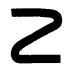
\includegraphics[keepaspectratio]{images/part002_9de8d58d.jpg}}

\begin{enumerate}
\def\labelenumi{\arabic{enumi})}
\setcounter{enumi}{1}
\tightlist
\item
  Let \((\theta_{\alpha})_{\alpha\in\mathbb{A}}\) be a family of complex measures on X; the family \((\theta_{\alpha})\) is said to be summable if the family \((|\theta_{\alpha}|)\) of positive measures is summable; it is not sufficient for this that the family \((\theta_{\alpha})\) be summable in the vector space \(\mathcal{M}(X;\mathbf{C})\) equipped with the vague topology (cf.~Exer. 3).
\end{enumerate}

\subsection{Integration with respect to a sum of positive measures}

Throughout this No., X denotes a locally compact space, \((\lambda_{\alpha})_{\alpha\in A}\) a summable family of positive measures on X, and \(\nu\) the measure \(\sum_{\alpha\in A}\lambda_{\alpha}\) .

PROPOSITION 1. --- Let \(f\) be a positive numerical function defined on \(X\) . Then

\[
\nu^ {\bullet} (f) = \sum_ {\alpha \in A} \lambda_ {\alpha} ^ {\bullet} (f).\tag{3}
\]

This follows at once from Remark 1, Prop. 11 of §1, No.~3 and Prop. 3 of §1, No.~1.

COROLLARY 1. --- For every compact (resp. open and relatively compact) subset M of X,

\[
\nu (\mathrm{M}) = \sum_ {\alpha \in \mathrm{A}} \lambda_ {\alpha} (\mathrm{M}).
\]

COROLLARY 2. --- For a subset N of X to be locally \(\nu\) -negligible, it is necessary and sufficient that, for every \(\alpha \in A\) , N be locally \(\lambda_{\alpha}\) -negligible.

COROLLARY 3. --- For every function \(f \in \mathcal{F}_{+}(X)\) ,

\[
\nu^ {*} (f) \geqslant \sum_ {\alpha \in A} \lambda_ {\alpha} ^ {*} (f).\tag{4}
\]

The inequality is obvious if \(f\) is not \(\nu\) -moderated, because then \(\nu^{*}(f) = +\infty\) (§1, No.~2, Prop. 7). If \(f\) is \(\nu\) -moderated then \(f\) is \(\lambda_{\alpha}\) -moderated for every \(\alpha \in A\) , because every \(\nu\) -integrable open set is \(\lambda_{\alpha}\) -integrable; the relation (4) then follows at once from (3) and from Prop. 7 of §1, No.~2.

\pandocbounded{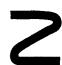
\includegraphics[keepaspectratio]{images/part002_632746ad.jpg}}

It can happen that the two members of (4) are not equal, even when A is countable and each of the \(\lambda_{\alpha}\) is a point measure ( \(\S 1\) , Exer. 4 \(a\) )).

PROPOSITION 2. --- Let f be a mapping of X into a topological space G. For f to be \(\nu\) -measurable, it is necessary and sufficient that f be \(\lambda_{\alpha}\) -measurable for every \(\alpha \in A\) .

This follows at once from Cor. 2 of Prop. 11 of §1.

PROPOSITION 3. --- For a mapping f of X into a Banach space F to be essentially \(\nu\) -integrable, it is necessary and sufficient that f be essentially \(\lambda_{\alpha}\) -integrable for every \(\alpha \in A\) and that

\[
\sum_ {\alpha \in \mathrm{A}} \int^ {\bullet} | \mathbf {f} | d \lambda_ {\alpha} <   + \infty .\tag{5}
\]

The family \((\int \mathbf{f}d\lambda_{\alpha})_{\alpha \in \mathrm{A}}\) is then absolutely summable in \(\mathrm{F}\) , and

\[
\int \mathbf {f} d \nu = \sum_ {\alpha \in \mathrm{A}} \int \mathbf {f} d \lambda_ {\alpha}.\tag{6}
\]

Indeed, for \(\mathbf{f}\) to be essentially \(\nu\) -integrable (resp. essentially \(\lambda_{\alpha}\) -integrable), it is necessary and sufficient that \(\mathbf{f}\) be measurable for the measure \(\nu\) (resp. \(\lambda_{\alpha}\) ) and that \(\nu^{\bullet}(|\mathbf{f}|) < +\infty\) (resp. \(\lambda_{\alpha}^{\bullet}(|\mathbf{f}|) < +\infty\) ), by virtue of Prop. 9 of §1, No.~3. The first part of the statement therefore follows at once from Props. 2 and 1. If \(\mathbf{f}\) is essentially \(\nu\) -integrable, the inequality

\[
\sum_ {\alpha \in \mathrm{A}} \left| \int \mathbf {f} d \lambda_ {\alpha} \right| \leqslant \sum_ {\alpha \in \mathrm{A}} \int | \mathbf {f} | d \lambda_ {\alpha} = \nu (| \mathbf {f} |)
\]

implies that the family \(\left(\int\mathbf{f}d\lambda_{\alpha}\right)\) is absolutely summable in F, and that the norm of the sum is less than or equal to the norm of f in \(\overline{\mathcal{L}}_{\mathrm{F}}^{1}(\nu)\) . The set of \(\mathbf{f}\in\mathcal{L}_{\mathrm{F}}^{1}(\nu)\) that satisfy (6) is thus a closed linear subspace H of \(\mathcal{L}_{\mathrm{F}}^{1}(\nu)\) ; now, this subspace is also dense in \(\mathcal{L}_{\mathrm{F}}^{1}(\nu)\) , because it contains the functions of the form \(f\cdot a\) , where \(a\in F\) and f denotes a finite integrable positive function (Prop. 1). Therefore \(\mathcal{H}=\mathcal{L}_{\mathrm{F}}^{1}(\nu)\) and the proposition is established.

Prop. 3 can also be deduced from the general theorem on integration that will be proved in §3 (No.~3, Th. 1).

COROLLARY 1. --- Suppose that f is \(\nu\) -integrable; then f is \(\lambda_{\alpha}\) -integrable for every \(\alpha \in A\) , and formula (6) holds. Conversely, if the set A is finite and f is \(\lambda_{\alpha}\) -integrable for every \(\alpha \in A\) , then the function f is \(\nu\) -integrable.

If \(\mathbf{f}\) is \(\nu\) -integrable, then \(\mathbf{f}\) is essentially \(\nu\) -integrable and \(\nu\) -moderated (§1, No.~3, Cor. of Prop. 9); \(\mathbf{f}\) is therefore essentially \(\lambda_{\alpha}\) -integrable and \(\lambda_{\alpha}\) -moderated, hence \(\lambda_{\alpha}\) -integrable, for every \(\alpha \in A\) . Conversely, if \(A\) is finite and if \(\mathbf{f}\) is \(\lambda_{\alpha}\) -integrable for all \(\alpha \in A\) , then \(\mathbf{f}\) is essentially \(\nu\) -integrable by Prop. 3, and it suffices to verify that \(\nu^{*}(|\mathbf{f}|) < +\infty\) ; this follows at once from the relation \(\nu^{*} = \sum_{\alpha \in A} \lambda_{\alpha}^{*}\) (Ch. IV, §1, No.~3, Prop. 15).

COROLLARY 2. --- Let \(\theta\) be a complex measure on X; set \(\theta_1 = (\mathcal{R}\theta)^+\) , \(\theta_2 = (\mathcal{R}\theta)^-\) , \(\theta_3 = (\mathcal{I}\theta)^+\) , \(\theta_4 = (\mathcal{I}\theta)^-\) . In order that a mapping \(f\) of X into a topological space G (resp. into a Banach space F) be measurable (resp. essentially integrable, integrable) for the measure \(\theta\) , it is necessary and sufficient that it be measurable (resp. essentially integrable, integrable) for each of the measures \(\theta_i\) ( \(i = 1,2,3,4\) ).

If f is measurable (resp. essentially integrable, integrable) for \(\theta\) , then f is by definition measurable (resp. essentially integrable, integrable) for the measure \(|\theta|\) , hence also for the measures \(\theta_{i}\) , which are \(\leqslant |\theta|\) . Conversely, if f is measurable (resp. essentially integrable, integrable) for the measures \(\theta_{i}\) , then Prop. 2 (resp. Prop. 3, Cor. 1 of Prop. 3) implies that f is measurable (resp. essentially integrable, integrable) for the measure \(\theta_{1} + \theta_{2} + \theta_{3} + \theta_{4}\) , which is \(\geqslant |\theta|\) .

\subsection{Decomposition of a measure as a sum of measures with compact support}

PROPOSITION 4. --- Let \(\mu\) be a positive measure on a locally compact space \(T\) , and let \(\mathfrak{K}\) be a \(\mu\) -dense set of compact subsets of \(T\) . There exists a summable family \((\mu_{\alpha})_{\alpha \in A}\) of positive measures on \(T\) such that \(\mu = \sum_{\alpha \in A} \mu_{\alpha}\) , and such that the supports of the measures \(\mu_{\alpha}\) belong to \(\mathfrak{K}\) and form a locally countable family of pairwise disjoint compact sets.

If the measure \(\mu\) is moderated, the index set A may be taken to be countable.

Consider a locally countable family \((\mathrm{K}_{\alpha})_{\alpha\in\mathrm{A}}\) of pairwise disjoint elements of K such that the set \(N = T - \bigcup K_{\alpha}\) is locally \(\mu\) -negligible (Ch. IV, §5, No.~9, Prop. 14). For every function \(f \in \mathcal{K}(\mathrm{T})\) , set

\[
\mu_ {\alpha} (f) = \mu (f \varphi_ {\mathrm{K} _ {\alpha}});
\]

the linear form \(\mu_{\alpha}\) on \(\mathcal{K}(\mathrm{T})\) is positive, therefore is a positive measure, with support contained in \(\mathrm{K}_{\alpha}\) . Since every compact set contained in an element of \(\mathfrak{K}\) belongs to \(\mathfrak{K}\) , \(\operatorname{Supp}(\mu_{\alpha}) \in \mathfrak{K}\) for all \(\alpha \in \mathrm{A}\) . It remains only to show that the family \((\mu_{\alpha})\) is summable and that its sum is equal to \(\mu\) , in other words that \(\sum_{\alpha \in \mathrm{A}} \mu_{\alpha}(f) = \mu(f)\) for every function \(f \in \mathcal{K}_{+}(\mathrm{T})\) . Now, let S be the (compact) support of \(f\) , and let \(\mathrm{A}'\) be the countable set formed by the \(\alpha \in \mathrm{A}\) such that \(\mathrm{S} \cap \mathrm{K}_{\alpha} \neq \varnothing\) . Since the set \(\mathrm{N} \cap \mathrm{S}\) is \(\mu\) -negligible,

\[
\begin{array}{c} \mu (f) = \mu (f \varphi_ {\mathrm{S}}) = \sum_ {\alpha \in \mathrm{A} ^ {\prime}} \mu (f \varphi_ {\mathrm{S} \cap \mathrm{K} _ {\alpha}}) = \sum_ {\alpha \in \mathrm{A} ^ {\prime}} \mu (f \varphi_ {\mathrm{K} _ {\alpha}}) \\ = \sum_ {\alpha \in \mathrm{A}} \mu (f \varphi_ {\mathrm{K} _ {\alpha}}) = \sum_ {\alpha \in \mathrm{A}} \mu_ {\alpha} (f). \end{array}
\]

This completes the proof of the general case. If \(\mu\) is moderated, then the set T is \(\mu\) -moderated and so T is the union of a sequence \((\mathrm{L}_n)\) of compact sets and a negligible set (§1, No.~2, Prop. 5); let \(\mathbf{A}'\) be the countable set of \(\alpha \in \mathbf{A}\) such that \(\mathrm{K}_{\alpha}\) intersects one of the \(\mathrm{L}_n\) . Then \(\mu_{\alpha} = 0\) for \(\alpha \notin \mathbf{A}'\) , and the last sentence of the statement follows immediately.

Remark. --- A positive measure may be the sum of a sequence of measures with compact support, and not be moderated (see Exer. 4 a) of §1).

\section{INTEGRATION OF POSITIVE MEASURES}

\subsection{Functions with values in a space of measures}

Let X be a locally compact space, \(\mathcal{M}_{+}(X)\) the convex cone of positive measures on X. Throughout the rest of this chapter, \(\mathcal{M}_{+}(X)\) will be equipped with the topology induced by the vague topology on \(\mathcal{M}(X)\) (Ch. III, §1, No.~9); thus, to say that a mapping \(\Lambda: t \mapsto \lambda_{t}\) of the locally compact space T into \(\mathcal{M}_{+}(X)\) is continuous means that, for every function \(f \in \mathcal{K}(X)\) , the numerical function \(t \mapsto \lambda_{t}(f)\) is continuous. In this case we shall also say that \(\Lambda\) is vaguely continuous on T. To say that a mapping \(\Lambda: t \mapsto \lambda_{t}\) is \(\mu\) -measurable means that the set of compact subsets K of T, such that the restriction of \(\Lambda\) to K is vaguely continuous, is \(\mu\) -dense (Ch. IV, §5, No.~10, Prop. 15). We shall then say that \(\Lambda\) is vaguely \(\mu\) -measurable.

Let \(\Lambda : t \mapsto \lambda_t\) be a mapping of T into \(\mathcal{M}_+(\mathrm{X})\) ; we shall say that \(\Lambda\) is scalarly essentially integrable for the measure \(\mu\) if, for every function \(f \in \mathcal{K}(\mathrm{X})\) , the function \(t \mapsto \lambda_t(f)\) is essentially \(\mu\) -integrable. If one sets \(\nu(f) = \int \lambda_t(f) d\mu(t)\) , it is clear that \(\nu\) is a positive linear form on \(\mathcal{K}(\mathrm{X})\) , hence is a measure on X (Ch. III, §1, No.~5, Th. 1). We will say that \(\nu\) is the integral of the function \(\Lambda\) with values in \(\mathcal{M}_+(\mathrm{X})\) , and we will write \(\nu = \int \lambda_t d\mu(t)\) .

The preceding definition is a special case of the concept of weak integral, which will be treated in a general manner in Ch. VI.

If \(f\) denotes an element of \(\mathcal{K}(\mathrm{X})\) , the integral \(\int \lambda_t(f) d\mu(t)\) will also, by an abuse of notation, be denoted \(\int d\mu(t) \int f(x) d\lambda_t(x)\) ; the definition of the integral \(\nu = \int \lambda_t d\mu(t)\) may then be written

\[
\int f (x) d \nu (x) = \int d \mu (t) \int f (x) d \lambda_ {t} (x).\tag{1}
\]

We shall make analogous abuses of notation in the sequel, for upper integrals, essential upper integrals, and integrals of functions with values in a Banach space.

Examples. --- 1) Suppose that T is a discrete space, and that \(\mu\) is the measure on T defined by placing a mass \(+1\) at each point of T (Ch. III, §1, No.~3). Let \(h\) be a function \(\geqslant 0\) defined on T; since the function \(h\) is lower semi-continuous (even continuous) on T, \(\mu^{*}(h) = \mu^{\bullet}(h) = \sum_{t\in \mathrm{T}}h(t)\) (Ch. IV, §1, No.~1, Example).

For the measure \(\mu\) , the notions of integrable function and essentially integrable function are therefore identical. This being so, to say that a mapping \(t \mapsto \lambda_t\) of T into \(\mathcal{M}_+(X)\) is scalarly essentially \(\mu\) -integrable amounts to saying that the family \((\lambda_t)_{t \in \mathrm{T}}\) is summable (§2, No.~1), and one then has \(\int \lambda_t d\mu(t) = \sum_{t \in \mathrm{T}} \lambda_t\) . Note that the mapping \(t \mapsto \lambda_t\) is vaguely continuous.

\begin{enumerate}
\def\labelenumi{\arabic{enumi})}
\setcounter{enumi}{1}
\tightlist
\item
  The mapping \(t \mapsto \varepsilon_t\) of \(T\) into \(\mathcal{M}_+(T)\) is vaguely continuous, scalarly essentially \(\mu\) -integrable for every positive measure \(\mu\) on \(T\) , and one has \(\int \varepsilon_t d\mu(t) = \mu\) .
\end{enumerate}

PROPOSITION 1. --- Suppose that \(\mu\) is the supremum of an increasing directed family \((\mu_i)_{i \in I}\) of positive measures on T; in order that \(\Lambda : t \mapsto \lambda_t\) be scalarly essentially \(\mu\) -integrable, it is necessary and sufficient that \(\Lambda\) be scalarly essentially \(\mu_i\) -integrable for all \(i \in I\) and that the family \(\left( \int \lambda_t d\mu_i(t) \right)_{i \in I}\) be bounded above in \(\mathcal{M}(X)\) . One then has,

\[
\int \lambda_ {t} d \mu (t) = \sup _ {i \in \mathrm{I}} \int \lambda_ {t} d \mu_ {i} (t).\tag{2}
\]

For, verifying that \(\Lambda\) is scalarly essentially integrable for a positive measure \(\eta\) on T comes down to verifying that \(t \mapsto \lambda_{t}(g)\) is \(\eta\) -measurable and admits a finite essential upper integral, with respect to \(\eta\) , for every function \(g \in \mathcal{K}_{+}(X)\) . The proposition therefore follows at once from Prop. 11 of §1, No.~4 and its Corollary 2.

COROLLARY. --- Suppose that \(\mu\) is the sum of a summable family \((\mu_{\alpha})_{\alpha \in \mathbf{A}}\) of positive measures on \(\mathbf{T}\) ; in order that \(\Lambda : t \mapsto \lambda_t\) be scalarly essentially \(\mu\) -integrable, it is necessary and sufficient that \(\Lambda\) be scalarly essentially \(\mu_{\alpha}\) -integrable for every \(\alpha \in \mathbf{A}\) and that the family of measures \(\int \lambda_t d\mu_{\alpha}(t)\) be summable. One then has

\[
\int \lambda_ {t} d \mu (t) = \sum_ {\alpha \in A} \int \lambda_ {t} d \mu_ {\alpha} (t).\tag{3}
\]

It follows immediately that every scalarly essentially \(\mu\) -integrable mapping is also scalarly essentially \(\mu'\) -integrable for every measure \(\mu' \leqslant \mu\) .

In this section we shall limit ourselves to the study of scalarly essentially integrable mappings of T into \(\mathcal{M}_{+}(X)\) that have the property contemplated in the following definition:

DEFINITION 1. --- Let X be a locally compact space, \(\Lambda : t \mapsto \lambda_t\) a scalarly essentially \(\mu\) -integrable mapping of T into \(\mathcal{M}_{+}(X)\) , and \(\nu\) the integral of \(\Lambda\) .

We say that \(\Lambda\) is \(\mu\) -pre-adequate if, for every lower semi-continuous function \(f \geqslant 0\) defined on X, the function \(t \mapsto \int^{\bullet} f d\lambda_t\) is \(\mu\) -measurable on T and

\[
\int^ {\bullet} f (x) d \nu (x) = \int^ {\bullet} d \mu (t) \int^ {\bullet} f (x) d \lambda_ {t} (x).\tag{4}
\]

We say that \(\Lambda\) is \(\mu\) -adequate (*) if \(\Lambda\) is \(\mu'\) -pre-adequate for every positive measure \(\mu' \leqslant \mu\) .

It can be shown that if \(\Lambda\) is \(\mu\) -pre-adequate and if the measure \(\nu = \int \lambda_{t} d\mu(t)\) is moderated---in particular if X is countable at infinity---then \(\Lambda\) is \(\mu\) -adequate (Exer. 7); however, it is not known if these concepts are in general equivalent. In the statements in Nos. 2 and 3 below, the assertions preceded by an a) or a b) extend at once to pre-adequate mappings, whereas those preceded by a c) are valid only for adequate mappings.

The following proposition often permits one to verify that a given mapping is \(\mu\) -adequate.

PROPOSITION 2. --- Let \(\Lambda : t \mapsto \lambda_t\) be a scalarly essentially \(\mu\) -integrable mapping of T into \(\mathcal{M}_{+}(X)\) , and let \(\nu = \int \lambda_t d\mu(t)\) .

\begin{enumerate}
\def\labelenumi{\alph{enumi})}
\tightlist
\item
  If \(\Lambda\) is vaguely continuous, then the mapping \(t \mapsto \lambda_t^\bullet(f)\) is lower semi-continuous for every lower semi-continuous function \(f \geqslant 0\) defined on X, \(\Lambda\) is \(\mu\) -adequate, and we have the relation
\end{enumerate}

\[
\int^ {*} f (x) d \nu (x) = \int^ {*} d \mu (t) \int^ {*} f (x) d \lambda_ {t} (x).\tag{5}
\]

\begin{enumerate}
\def\labelenumi{\alph{enumi})}
\setcounter{enumi}{1}
\item
  If \(\Lambda\) is vaguely \(\mu\) -measurable, then \(\Lambda\) is \(\mu\) -adequate.
\item
  If the topology of X admits a countable base, then \(\Lambda\) is vaguely \(\mu\) -measurable (hence also \(\mu\) -adequate).
\end{enumerate}

Let \(f\) be a lower semi-continuous function \(\geqslant 0\) defined on \(X\) . Let \(F\) be the set, directed for the relation \(\leqslant\) , of functions \(g \in \mathcal{H}(X)\) such that \(0 \leqslant g \leqslant f\) . For \(g \in F\) , denote by \(h_g\) the function defined on \(T\) by \(h_g(t) = \lambda_t(g)\) . Similarly, set

\[
h _ {f} (t) = \lambda_ {t} ^ {*} (f) = \lambda_ {t} ^ {\bullet} (f) = \sup _ {g \in \mathrm{F}} h _ {g} (t)
\]

(§1, No.~1, Prop. 4). Let us make the following hypothesis, weaker than that of a): assume only that the restriction of \(\Lambda\) to S is vaguely continuous, where S is a closed subset of T that contains the support of \(\mu\) . For \(g \in \mathbf{F}\) , denote by \(\overline{h}_g\) the numerical function that coincides with \(h_g\) on S and has the value \(+\infty\) on \(\mathbb{C}S\) . Set \(\overline{h}_f = \sup_{g \in \mathbb{F}} \overline{h}_g\) ; then \(\overline{h}_f = h_f\) on S. For every \(g \in \mathbf{F}\) , the function \(\overline{h}_g\) is lower semi-continuous; \(\overline{h}_f\) is therefore lower semi-continuous and, since the family \((\overline{h}_g)_{g \in \mathbb{F}}\) is directed,

\[
\mu^ {*} (\overline {{h}} _ {f}) = \sup _ {g \in \mathrm{F}} \mu^ {*} (\overline {{h}} _ {g}) = \sup _ {g \in \mathrm{F}} \mu^ {*} (h _ {g}) = \sup _ {g \in \mathrm{F}} \nu (g) = \nu^ {*} (f)
\]

(Ch. IV, §1, No.~1, Th. 1 and §2, No.~3, Prop. 6). Since \(h_f = \overline{h}_f\) on S, hence almost everywhere, this may also be written \(\mu^*(h_f) = \nu^*(f)\) , an equality identical to (5). Similarly, \(f\) and \(\overline{h}_f\) being lower semi-continuous, the preceding relations yield the equality \(\mu^\bullet(\overline{h}_f) = \nu^\bullet(f)\) (§1, No.~1, Prop. 4); since \(\overline{h}_f = h_f\) on S, it follows that \(\mu^\bullet(h_f) = \nu^\bullet(f)\) (§1, No.~1, Prop. 1), an equality identical to (4). The mapping \(\Lambda\) is therefore \(\mu\) -pre-adequate; but one could have replaced everywhere in this argument \(\mu\) by \(\mu' \leqslant \mu\) , and \(\nu\) by \(\nu' = \int \lambda_t d\mu'(t)\) , because \(\Lambda\) is also scalarly essentially \(\mu'\) -integrable and S contains the support of \(\mu'\) . It follows from this that \(\Lambda\) is \(\mu\) -adequate.

Suppose \(\Lambda\) is vaguely continuous; we may take \(S = T\) ; then \(h_f = \overline{h}_f\) is lower semi-continuous, which completes the proof of part a) of the statement.

Assume that \(\Lambda\) is vaguely \(\mu\) -measurable and let us prove b). The set \(\mathfrak{K}\) of compact subsets K of T such that the restriction of \(\Lambda\) to K is continuous being \(\mu\) -dense (Ch. IV, §5, No.~10, Prop. 15), there exists a summable family \((\mu_{\alpha})_{\alpha \in \mathrm{A}}\) of measures on T such that \(\mu = \sum_{\alpha \in \mathrm{A}} \mu_{\alpha}\) and the support of each of the measures \(\mu_{\alpha}\) belongs to \(\mathfrak{K}\) (§2, No.~3, Prop. 4). For every \(\alpha \in \mathrm{A}\) , the mapping \(\Lambda\) is scalarly essentially \(\mu_{\alpha}\) -integrable, and we set \(\nu_{\alpha} = \int \lambda_t d\mu_{\alpha}(t)\) ; the family \((\nu_{\alpha})\) is summable, and its sum is equal to \(\nu\) (Cor. of Prop. 1). If \(f\) is a positive lower semi-continuous function defined on X, the first part of the proof, applied to the measures \(\mu_{\alpha}\) and the closed sets \(S_{\alpha}\) , shows that:

\(1^{\circ} h_{f}\) is \(\mu_{\alpha}\) -measurable for every \(\alpha \in A\) , hence is \(\mu\) -measurable (§2, No.~2, Prop. 2), and

\[
2 ^ {\circ} \int^ {\bullet} f (x) d \nu_ {\alpha} (x) = \int^ {\bullet} d \mu_ {\alpha} (t) \int^ {\bullet} f (x) d \lambda_ {t} (x).
\]

The formula (4) follows on summing over \(\alpha\) ( \(\S 2\) , No.~2, Prop. 1). Applying the preceding argument to an arbitrary measure \(\mu' \leqslant \mu\) (which is legitimate, since \(\Lambda\) is scalarly essentially \(\mu'\) -integrable and vaguely \(\mu'\) -measurable, cf.~\(\S 2\) , No.~2, Prop. 2), we conclude that \(\Lambda\) is \(\mu'\) -pre-adequate, and b) is proved.

Finally, assuming that the topology of X admits a countable base, let us show that every scalarly essentially \(\mu\) -integrable mapping \(\Lambda: t \mapsto \lambda_{t}\) of T into \(\mathcal{M}_{+}(X)\) is vaguely \(\mu\) -measurable. This will result from the following lemma:

Lemma. --- Let X be a locally compact space having a countable base. Then, there exists in \(\mathcal{K}(\mathrm{X})\) a countable subset S having the following property: for every function \(f \in \mathcal{K}(\mathrm{X})\) , there exist a sequence \((f_n)\) of elements of S and a positive function \(\varphi \in S\) such that, for every number \(\varepsilon > 0\) , \(|f_n - f| \leqslant \varepsilon \varphi\) provided n is sufficiently large.

Let \(X'\) be the Alexandroff compactification of \(X\) , which is a metrizable compact space (GT, IX, §2, No.~9, Prop. 16 and Cor.); we identify \(\mathcal{K}(X)\) with a subset of \(\mathcal{C}(X')\) . Let \(S'\) be a countable dense subset of the Banach space \(\mathcal{C}(X')\) (GT, X, §3, No.~3, Th. 1); we can suppose that \(S'\) contains the constant function \(n\) for every \(n \in N\) . Let \((U_n)\) be a sequence of relatively compact open sets in \(X\) , with union \(X\) , such that \(\overline{U}_n \subset U_{n+1}\) for all \(n\) (GT, I, §9, No.~9, Prop. 15), and let \(\varphi_n\) be a function in \(\mathcal{K}_+(X)\) equal to 1 on \(\overline{U}_n\) . We denote by \(S\) the countable set of elements of \(\mathcal{K}(X)\) of the form \(\varphi_n g\) ( \(n \in N, g \in S'\) ). If \(f \in \mathcal{K}(X)\) , let \((g_n)\) be a sequence of elements of \(S'\) that converges uniformly to \(f\) , and let \(k\) be an integer such that the support of \(f\) is contained in \(U_k\) . Finally, let \(m\) be an integer that is an upper bound for the norms of the functions \(g_n\) . The functions \(f_n = \varphi_k g_n\) belong to \(S\) and satisfy the statement, with \(\varphi = m\varphi_k\) .

The lemma having been established, and the mapping \(t \mapsto \lambda_t(g)\) being essentially \(\mu\) -integrable for every \(g \in S\) , the mapping \(t \mapsto (\lambda_t(g))_{g \in S}\) of \(T\) into \(\mathbf{R}^S\) is \(\mu\) -measurable (Ch. IV, §5, No.~3, Th. 1). The set \(\mathfrak{K}\) , of compact subsets \(K\) of \(T\) such that the restriction of this mapping to \(K\) is continuous, is therefore \(\mu\) -dense, and it will suffice to show that the restriction of \(\Lambda\) to every \(K \in \mathfrak{K}\) is continuous. Now, let \(f\) be any element of \(\mathcal{H}(X)\) , \(f_n\) and \(\varphi\) elements of \(S\) satisfying the statement of the Lemma; the function \(t \mapsto \lambda_t(f)\) is then the uniform limit on \(K\) of the continuous functions \(t \mapsto \lambda_t(f_n)\) ; it is therefore continuous on \(K\) , and the proposition is proved.
